\documentclass[11pt,a4paper,twoside]{book}
\usepackage[]{graphicx}\usepackage[]{color}
%% maxwidth is the original width if it is less than linewidth
%% otherwise use linewidth (to make sure the graphics do not exceed the margin)
\makeatletter
\def\maxwidth{ %
  \ifdim\Gin@nat@width>\linewidth
    \linewidth
  \else
    \Gin@nat@width
  \fi
}
\makeatother

\definecolor{fgcolor}{rgb}{0.345, 0.345, 0.345}
\newcommand{\hlnum}[1]{\textcolor[rgb]{0.686,0.059,0.569}{#1}}%
\newcommand{\hlstr}[1]{\textcolor[rgb]{0.192,0.494,0.8}{#1}}%
\newcommand{\hlcom}[1]{\textcolor[rgb]{0.678,0.584,0.686}{\textit{#1}}}%
\newcommand{\hlopt}[1]{\textcolor[rgb]{0,0,0}{#1}}%
\newcommand{\hlstd}[1]{\textcolor[rgb]{0.345,0.345,0.345}{#1}}%
\newcommand{\hlkwa}[1]{\textcolor[rgb]{0.161,0.373,0.58}{\textbf{#1}}}%
\newcommand{\hlkwb}[1]{\textcolor[rgb]{0.69,0.353,0.396}{#1}}%
\newcommand{\hlkwc}[1]{\textcolor[rgb]{0.333,0.667,0.333}{#1}}%
\newcommand{\hlkwd}[1]{\textcolor[rgb]{0.737,0.353,0.396}{\textbf{#1}}}%
\let\hlipl\hlkwb

\usepackage{framed}
\makeatletter
\newenvironment{kframe}{%
 \def\at@end@of@kframe{}%
 \ifinner\ifhmode%
  \def\at@end@of@kframe{\end{minipage}}%
  \begin{minipage}{\columnwidth}%
 \fi\fi%
 \def\FrameCommand##1{\hskip\@totalleftmargin \hskip-\fboxsep
 \colorbox{shadecolor}{##1}\hskip-\fboxsep
     % There is no \\@totalrightmargin, so:
     \hskip-\linewidth \hskip-\@totalleftmargin \hskip\columnwidth}%
 \MakeFramed {\advance\hsize-\width
   \@totalleftmargin\z@ \linewidth\hsize
   \@setminipage}}%
 {\par\unskip\endMakeFramed%
 \at@end@of@kframe}
\makeatother

\definecolor{shadecolor}{rgb}{.97, .97, .97}
\definecolor{messagecolor}{rgb}{0, 0, 0}
\definecolor{warningcolor}{rgb}{1, 0, 1}
\definecolor{errorcolor}{rgb}{1, 0, 0}
\newenvironment{knitrout}{}{} % an empty environment to be redefined in TeX

\usepackage{alltt}
\newcommand{\SweaveOpts}[1]{}  % do not interfere with LaTeX
\newcommand{\SweaveInput}[1]{} % because they are not real TeX commands
\newcommand{\Sexpr}[1]{}       % will only be parsed by R


% We load package by package and set package relevant parameters.
% Topics are summarized later
%%%%%%%%%%%%%%%%%%%%%%%%%%%%%%%%%%%%%%%%%%%%%%%%%%%%%%%%%%%%%%%%%%%%%%%%
% helping packages
\usepackage{ifthen}
\usepackage{calc}

\usepackage[T1]{fontenc}       % provides fonts having  accented characters 
\usepackage[latin1]{inputenc}  % allows the user to input accented characters directly from the keyboard

%%%%%%%%%%%%%%%%%%%%%%%%%%%%%%%%%%%%%%%%%%%%%%%%%%%%%%%%%%%%%%%%%%%%%%%%

\renewcommand{\baselinestretch}{1.2}
\renewcommand{\textfraction}{0}%0.2     % placement of figures
\renewcommand{\topfraction}{1}%.3
\renewcommand{\bottomfraction}{1}%.3
\renewcommand{\floatpagefraction}{1}%.3
\setcounter{bottomnumber}{3}%1

\textwidth6.3in
\textheight9.7in
\topmargin-45pt
\oddsidemargin-.15in
\evensidemargin.15in
\headsep30pt
\headheight15pt
%\footskip20pt


%%%%%%%%%%%%%%%%%%%%%%%%%%%%%%%%%%%%%%%%%%%%%%%%%%%%%%%%%%%%%%%%%%%%%%%%

\usepackage[dvipsnames]{xcolor}
\definecolor{fgcolor}{rgb}{0.345, 0.345, 0.345}
\definecolor{shadecolor}{rgb}{.97, .97, .97}
\definecolor{messagecolor}{rgb}{0, 0, 0}
\definecolor{warningcolor}{rgb}{1, 0, 1}
\definecolor{errorcolor}{rgb}{1, 0, 0}
\definecolor{DarkBlue}{rgb}{0,0,0.5451}
\definecolor{DarkGreen}{rgb}{0,0.39216,0}
\definecolor{LightYellow}{rgb}{1,1,.8}
\definecolor{orange}{rgb}{.9,0.3445,0}



%%%%%%%%%%%%%%%%%%%%%%%%%%%%%%%%%%%%%%%%%%%%%%%%%%%%%%%%%%%%%%%%%%%%%%%%
\usepackage{afterpage}
\usepackage{natbib}
\usepackage{upquote}

\usepackage[english]{babel}

%%%%%%%%%%%%%%%%%%%%%%%%%%%%%%%%%%%%%%%%%%%%%%%%%%%%%%%%%%%%%%%%%%%%%%%%%%%%%%%
%% maxwidth is the original width if it is less than linewidth
%% otherwise use linewidth (to make sure the graphics do not exceed the margin)
\makeatletter
\def\maxwidth{ %
  \ifdim\Gin@nat@width>\linewidth
    \linewidth
  \else
    \Gin@nat@width
  \fi
}
\makeatother

%%%%%%%%%%%%%%%%%%%%%%%%%%%%%%%%%%%%%%%%%%%%%%%%%%%%%%%%%%%%%%%%%%%%%%%%%%%%%%%%%%%%%%%%%%%%%%%%%%%%%%%%%%%%
% from fancyvrb
\usepackage{fancyhdr}
\usepackage{fancyvrb}
\DefineVerbatimEnvironment{Rcode}{Verbatim}{xleftmargin=2em,fontshape=sl,formatcom=\color{DarkGreen}}
\fvset{listparameters={\setlength{\topsep}{0pt}}}

%%%%%%%%%%%%%%%%%%%%%%%%%%%%%%%%%%%%%%%%%%%%%%%%%%%%%%%%%%%%%%%%%%%%%%%%%%%%%%%%%%%%%%%%%%%%%%%%%%%%%%%%%%%%%
\usepackage{float}
\usepackage{graphicx}
\usepackage[margin=2em,labelfont=bf]{caption}


%%%%%%%%%%%%%%%%%%%%%%%%%%%%%%%%%%%%%%%%%%%%%%%%%%%%%%%%%%%%%%%%%%%%%%%%
\usepackage[pdftex,plainpages=false,pdfpagelabels,pagebackref=true,colorlinks=true,pdfpagemode=UseOutlines]{hyperref}


%%%%%%%%
\usepackage{tabularx}
%%%%%%%%

%%%%%%%%%%%%%%%%%%%%%%%%%%%%%%%%%%%%%%%%%%%%%%%%%%%%%%%%%%%%%%%%%%%%%%%%
% now math stuff and other details...
\usepackage{amsmath,amsthm,amssymb}

\newtheorem{pro}{Property}[chapter]
\theoremstyle{definition}
\newtheorem{des}{Definition}[chapter]
\newtheorem{bsp}{Example}[chapter]
\newtheorem{rem}{Remark}[chapter]

\newcommand*\widebar[1]{%
  \vbox{%
    \hrule height 0.5pt%     % Line above with certain width
    \kern0.5ex%             % Distance between line and content
    \hbox{%
      \kern-0.1em%           % Distance between content and left side of box, negative values for lines shorter than content
      \ifmmode#1\else\ensuremath{#1}\fi%  % The content, typeset in dependence of mode
      \kern-0.1em%      % Distance between content and left side of box, negative values for lines shorter than content
    }% end of hbox
  }% end of vbox
}
\def\ds{\displaystyle}

\newcommand{\rr}[1]{{\ttfamily\slshape\color{DarkGreen} #1}}

\makeatletter


% clever trick to circumvent potential redefines after loading packages:
% \providecommand{\something}{}  % if it does not exist, it creates it.
%      has same syntax as \newcommand
% \renewcommand{\something}{....}
% TUGboat 29(2)


\makeatletter
%umdefinierung exisitierender befehle
\let\oldH\H
\let\oldL\L
\let\oldO\H
\let\oldS\S
\let\olda\a
\let\oldb\b
\let\oldc\c
\let\oldd\d
\let\oldk\k
\let\oldv\v
\let\oldl\l
\let\oldt\t
\let\oldu\u
\let\oldIJ\IJ
\let\oldP\P
\let\P\relax
\let\oldnorm\|

%\DefineVerbatimEnvironment{CodeInput}{Verbatim}{fontshape=sl}
%\DefineVerbatimEnvironment{CodeOutput}{Verbatim}{}

% some classical environments, up-right, with chapter numbering.
\theoremstyle{definition}
\newtheorem{definition}{Definition}[chapter]
\newtheorem{example}{Example}[chapter]
\newtheorem{remark}{Remark}[chapter]
\newtheorem{theorem}{Theorem}[chapter]



\renewcommand{\|}{|\!|}         % closer norm
\newcommand{\T}{{}^{\top}}
\newcommand\code[1]{{\tt#1}}



\newcounter{algo}
\newenvironment{algorithm}{%
  \begin{list}{
      (\arabic{algo})
    }{
      \usecounter{algo}
    }%
}{
  \end{list}
}

% some text abbreviation
\newcommand{\GLS}{\text{GLS}}
\newcommand{\RR}{\text{RR}}
\newcommand{\OR}{\text{OR}}
\newcommand{\WLS}{\text{WLS}}
\newcommand{\MLE}{\text{MLE}}
\newcommand{\OLS}{\text{OLS}}
\newcommand{\MAE}{\text{MAE}}
\newcommand{\MAD}{\text{MAD}}
\newcommand{\RMSE}{\text{RMSE}}
\newcommand{\SVAR}{\text{svar}} %silvanos new commands
\newcommand{\EVAR}{\text{evar}}
\newcommand{\LMG}{\text{LMG}}
\newcommand{\Rtwo}{\text{R}^2}



\newcommand{\ii}{\text{\i}}

\newcommand{\Bin}{\cB\mathit{\!i\!n}}
\newcommand{\Beta}{\cB\mathit{\!e\!t\!a}}
\newcommand{\Pois}{\cP\mathit{\!o\!i\!s\!s\!o\!n}}
\newcommand{\Exp}{\cE\mathit{\!x\!p}}


\DeclareMathOperator*{\argmin}{argmin}
\DeclareMathOperator*{\argmax}{argmax}
\DeclareMathOperator{\diag}{diag}
\DeclareMathOperator{\diam}{diam}
\DeclareMathOperator{\card}{card}
\DeclareMathOperator{\cov}{Cov}                   
\DeclareMathOperator{\corr}{Corr}                 
\DeclareMathOperator{\var}{Var}                   
\DeclareMathOperator{\trace}{tr}                  
\DeclareMathOperator{\E}{E}                       
\DeclareMathOperator{\P}{P}                       
\DeclareMathOperator{\pred}{p}
\DeclareMathOperator{\vect}{vec}                  
\DeclareMathOperator{\vech}{vech}                 
\DeclareMathOperator{\rank}{rank}                 
\DeclareMathOperator{\e}{e}                       
%\DeclareMathOperator{\cv}{CV}                     
\DeclareMathOperator{\GCV}{GCV}                     
\DeclareMathOperator{\CV}{CV}                     
\DeclareMathOperator{\BLUP}{BLUP}                 
\DeclareMathOperator{\MSE}{MSE}                   
\DeclareMathOperator{\MS}{MS}                   
\DeclareMathOperator{\df}{df}                   
\DeclareMathOperator{\bias}{bias}                   
\DeclareMathOperator{\eig}{eig}                   
\DeclareMathOperator{\Prec}{Prec}
\DeclareMathOperator{\mode}{mode}
\renewcommand{\SS}{\text{SS}}
\renewcommand{\d}{\mathsf{\,d}}

\def\arctanh{\qopname\relax o{arctanh}}  % as in amsopn
\newcommand{\bigo}{\cO}
\newcommand{\lito}{\text{\scriptsize{$\cO$}}}
\newcommand{\cdfPhi}{\itPhi}
\newcommand{\ml}{_\text{ML}}

\newcommand*{\stack@relbin}[3][]{%
  \mathop{#3}\limits
  \toks@{#1}%
  \edef\reserved@a{\the\toks@}%
  \ifx\reserved@a\@empty\else_{#1}\fi
  \toks@{#2}%
  \edef\reserved@a{\the\toks@}%
  \ifx\reserved@a\@empty\else^{#2}\fi
  \egroup
}%
\renewcommand*{\stackrel}{\mathrel\bgroup\stack@relbin}
\newcommand*{\stackbin}{\mathbin\bgroup\stack@relbin}
\newcommand{\simiid}{\stackrel[]{\text{iid}}{\sim}}

% Kalligraphischer Schriftsatz
\newcommand{\cA}{{\cal{A}}}
\newcommand{\cB}{{\cal{B}}} 
\newcommand{\cC}{{\cal{C}}}
\newcommand{\cD}{{\cal{D}}} 
\newcommand{\cE}{{\cal{E}}}
\newcommand{\cF}{{\cal{F}}}
\newcommand{\cG}{{\cal{G}}}
\newcommand{\cH}{{\cal{H}}}
\newcommand{\cI}{{\cal{I}}}
\newcommand{\cJ}{{\cal{J}}}
\newcommand{\cK}{{\cal{K}}}
\newcommand{\cL}{{\cal{L}}}
\newcommand{\cM}{{\cal{M}}} 
\newcommand{\cN}{{\cal{N}}}
\newcommand{\cO}{{\cal{O}}} 
\newcommand{\cP}{{\cal{P}}}
\newcommand{\cQ}{{\cal{Q}}} 
\newcommand{\cR}{{\cal{R}}} 
\newcommand{\cS}{{\cal{S}}} 
\newcommand{\cT}{{\cal{T}}}
\newcommand{\cU}{{\cal{U}}}
\newcommand{\cV}{{\cal{V}}}
\newcommand{\cW}{{\cal{W}}}
\newcommand{\cX}{{\cal{X}}} 
\newcommand{\cY}{{\cal{Y}}}
\newcommand{\cZ}{{\cal{Z}}} 


\newcommand{\IA}{{\mathbb{A}}}
\newcommand{\IB}{{\mathbb{B}}}
\newcommand{\IC}{{\mathbb{C}}}
\newcommand{\ID}{{\mathbb{D}}}
\newcommand{\IE}{{\mathbb{E}}}
\newcommand{\IF}{{\mathbb{F}}}
\newcommand{\IG}{{\mathbb{G}}}
\newcommand{\IH}{{\mathbb{H}}}
\newcommand{\II}{{\mathbb{I}}}
%\newcommand{\IJ}{{\mathbb{J}}}
\newcommand{\IK}{{\mathbb{K}}}
\newcommand{\IL}{{\mathbb{L}}}
\newcommand{\IM}{{\mathbb{M}}}
\newcommand{\IN}{{\mathbb{N}}}
\newcommand{\IO}{{\mathbb{O}}}
\newcommand{\IP}{{\mathbb{P}}}
\newcommand{\IQ}{{\mathbb{Q}}}
\newcommand{\IR}{{\mathbb{R}}}
\newcommand{\IS}{{\mathbb{S}}}
\newcommand{\IT}{{\mathbb{T}}}
\newcommand{\IU}{{\mathbb{U}}}
\newcommand{\IV}{{\mathbb{V}}}
\newcommand{\IW}{{\mathbb{W}}}
\newcommand{\IX}{{\mathbb{X}}}
\newcommand{\IY}{{\mathbb{Y}}}
\newcommand{\IZ}{{\mathbb{Z}}}


% fette griechische kleinbuchstaben
\newcommand{\balpha}{{\boldsymbol{\alpha}}}
\newcommand{\bbeta}{{\boldsymbol{\beta}}}
\newcommand{\bgamma}{{\boldsymbol{\gamma}}}
\newcommand{\bdelta}{{\boldsymbol{\delta}}}
\newcommand{\blambda}{{\boldsymbol{\lambda}}}
\newcommand{\bepsilon}{{\boldsymbol{\epsilon}}}
\newcommand{\bvarepsilon}{{\boldsymbol{\varepsilon}}}
\newcommand{\bzeta}{{\boldsymbol{\zeta}}}
\newcommand{\bfeta}{{\boldsymbol{\eta}}}  %  <----- exception !
\newcommand{\btheta}{{\boldsymbol{\theta}}{}}
\newcommand{\bvartheta}{{\boldsymbol{\vartheta}}}
\newcommand{\biota}{{\boldsymbol{\iota}}}
\newcommand{\bkappa}{{\boldsymbol{\kappa}}}
\newcommand{\bmu}{{\boldsymbol{\mu}}}
\newcommand{\bnu}{{\boldsymbol{\nu}}}
\newcommand{\bxi}{{\boldsymbol{\xi}}}
\newcommand{\bpi}{{\boldsymbol{\pi}}}
\newcommand{\bvarpi}{{\boldsymbol{\varpi}}}
\newcommand{\brho}{{\boldsymbol{\rho}}}
\newcommand{\bvarrhoi}{{\boldsymbol{\varrho}}}
\newcommand{\bsigma}{{\boldsymbol{\sigma}}}
\newcommand{\bvarsigma}{{\boldsymbol{\varsigma}}}
\newcommand{\btau}{{\boldsymbol{\tau}}}
\newcommand{\bvartau}{{\boldsymbol{\vartau}}}
\newcommand{\bupsilon}{{\boldsymbol{\upsilon}}}
\newcommand{\bphi}{{\boldsymbol{\phi}}}
\newcommand{\bvarphi}{{\boldsymbol{\varphi}}}
\newcommand{\bchi}{{\boldsymbol{\chi}}}
\newcommand{\bpsi}{{\boldsymbol{\psi}}}
\newcommand{\bomega}{{\boldsymbol{\omega}}}


% fette griechische grossbuchstaben
\newcommand{\bGamma}{{\boldsymbol{\Gamma}}}
\newcommand{\bDelta}{{\boldsymbol{\Delta}}}
\newcommand{\bTheta}{{\boldsymbol{\Theta}}}
\newcommand{\bLambda}{{\boldsymbol{\Lambda}}{}}
\newcommand{\bXi}{{\boldsymbol{\Xi}}}
\newcommand{\bPi}{{\boldsymbol{\Pi}}}
\newcommand{\bSigma}{{\boldsymbol{\Sigma}}{}}
\newcommand{\bUpsilon}{{\boldsymbol{\Upsilon}}{}}
\newcommand{\bPhi}{{\boldsymbol{\Phi}}}
\newcommand{\bPsi}{{\boldsymbol{\Psi}}}
\newcommand{\bOmega}{{\boldsymbol{\Omega}}}

% italics griechische grossbuchstaben
\newcommand{\itGamma}{{\mathit{\Gamma}}}
\newcommand{\itDelta}{{\mathit{\Delta}}}
\newcommand{\itTheta}{{\mathit{\Theta}}}
\newcommand{\itLambda}{{\mathit{\Lambda}}}
\newcommand{\itXi}{{\mathit{\Xi}}}
\newcommand{\itPi}{{\mathit{\Pi}}}
\newcommand{\itSigma}{{\mathit{\Sigma}}}
\newcommand{\itUpsilon}{{\mathit{\Upsilon}}}
\newcommand{\itPhi}{{\mathit{\Phi}}}
\newcommand{\itPsi}{{\mathit{\Psi}}}
\newcommand{\itOmega}{{\mathit{\Omega}}}



\newcommand{\A}{{\mathbf{A}}}
\newcommand{\B}{{\mathbf{B}}}
\newcommand{\C}{{\mathbf{C}}}
\newcommand{\D}{{\mathbf{D}}}
\newcommand{\bfE}{{\mathbf{E}}}    % \E: expectation
\newcommand{\F}{{\mathbf{F}}}
\newcommand{\G}{{\mathbf{G}}}
\renewcommand{\H}{{\mathbf{H}}}
\newcommand{\I}{{\mathbf{I}}}
\newcommand{\J}{{\mathbf{J}}}
\newcommand{\K}{{\mathbf{K}}}
\renewcommand{\L}{{\mathbf{L}}}
\newcommand{\bfM}{{\mathbf{M}}}
\newcommand{\N}{{\mathbf{N}}}
\renewcommand{\O}{{\mathbf{O}}}
\newcommand{\bfP}{{\mathbf{P}}}  % \P : probability
\newcommand{\Q}{{\mathbf{Q}}}
\newcommand{\bfR}{{\mathbf{R}}}
\renewcommand{\S}{{\mathbf{S}}}
\newcommand{\bfT}{{\mathbf{T}}} % \T transpose
\newcommand{\U}{{\mathbf{U}}}
\newcommand{\V}{{\mathbf{V}}}
\newcommand{\W}{{\mathbf{W}}}
\newcommand{\X}{{\mathbf{X}}}
\newcommand{\Y}{{\mathbf{Y}}}
\newcommand{\Z}{{\mathbf{Z}}}


\newcommand{\0}{{\mathbf{0}}}
\newcommand{\1}{{\mathbf{1}}}
\newcommand{\2}{{\mathbf{2}}}
\newcommand{\3}{{\mathbf{3}}}
\newcommand{\4}{{\mathbf{4}}}
\newcommand{\5}{{\mathbf{5}}}
\newcommand{\6}{{\mathbf{6}}}
\newcommand{\7}{{\mathbf{7}}}
\newcommand{\8}{{\mathbf{8}}}
\newcommand{\9}{{\mathbf{9}}}

\renewcommand{\a}{{\textbf{\textit{a}}}}
\renewcommand{\b}{{\textbf{\textit{b}}}}
\renewcommand{\c}{{\textbf{\textit{c}}}}
\newcommand{\bfd}{{\textbf{\textit{d}}}}  % \d  'dx'
\newcommand{\bfe}{{\textbf{\textit{e}}}}  % \e  l'exponentiel
\newcommand{\f}{{\textbf{\textit{f}}}}
\newcommand{\g}{{\textbf{\textit{g}}}}
\newcommand{\h}{{\textbf{\textit{h}}}}
\newcommand{\bfi}{{\textbf{\textit{i}}}}%\i  complex i, sans 'dot'
\newcommand{\bfj}{{\textbf{\textit{j}}}}
\renewcommand{\l}{{\textbf{\textit{l}}}}
\renewcommand{\k}{{\textbf{\textit{k}}}}
\newcommand{\m}{{\textbf{\textit{m}}}}
\newcommand{\bfn}{{\textbf{\textit{n}}}}
\newcommand{\bfo}{{\textbf{\textit{o}}}}
\newcommand{\p}{{\textbf{\textit{p}}}}
\newcommand{\q}{{\textbf{\textit{q}}}}
\renewcommand{\r}{{\textbf{\textit{r}}}}
\newcommand{\s}{{\textbf{\textit{s}}}}
\renewcommand{\t}{{\textbf{\textit{t}}}}
\newcommand{\bfu}{{\textbf{\textit{u}}}} %\u used in references
\renewcommand{\v}{{\textbf{\textit{v}}}}
\newcommand{\w}{{\textbf{\textit{w}}}}
\newcommand{\x}{{\textbf{\textit{x}}}}
\newcommand{\y}{{\textbf{\textit{y}}}}
\newcommand{\z}{{\textbf{\textit{z}}}}




\ifcsname hlkwd\endcsname%    ... command '#1' exists ...%
\else%  ... command '#1' does not exist ...%

\def\maxwidth{ %
  \ifdim\Gin@nat@width>\linewidth
    \linewidth
  \else
    \Gin@nat@width
  \fi
}

\definecolor{fgcolor}{rgb}{0.345, 0.345, 0.345}
\newcommand{\hlnum}[1]{\textcolor[rgb]{0.686,0.059,0.569}{#1}}%
\newcommand{\hlstr}[1]{\textcolor[rgb]{0.192,0.494,0.8}{#1}}%
\newcommand{\hlcom}[1]{\textcolor[rgb]{0.678,0.584,0.686}{\textit{#1}}}%
\newcommand{\hlopt}[1]{\textcolor[rgb]{0,0,0}{#1}}%
\newcommand{\hlstd}[1]{\textcolor[rgb]{0.345,0.345,0.345}{#1}}%
\newcommand{\hlkwa}[1]{\textcolor[rgb]{0.161,0.373,0.58}{\textbf{#1}}}%
\newcommand{\hlkwb}[1]{\textcolor[rgb]{0.69,0.353,0.396}{#1}}%
\newcommand{\hlkwc}[1]{\textcolor[rgb]{0.333,0.667,0.333}{#1}}%
\newcommand{\hlkwd}[1]{\textcolor[rgb]{0.737,0.353,0.396}{\textbf{#1}}}%

\usepackage{framed}
\newenvironment{kframe}{%
 \def\at@end@of@kframe{}%
 \ifinner\ifhmode%
  \def\at@end@of@kframe{\end{minipage}}%
  \begin{minipage}{\columnwidth}%
 \fi\fi%
 \def\FrameCommand##1{\hskip\@totalleftmargin \hskip-\fboxsep
 \colorbox{shadecolor}{##1}\hskip-\fboxsep
     % There is no \\@totalrightmargin, so:
     \hskip-\linewidth \hskip-\@totalleftmargin \hskip\columnwidth}%
 \MakeFramed {\advance\hsize-\width
   \@totalleftmargin\z@ \linewidth\hsize
   \@setminipage}}%
 {\par\unskip\endMakeFramed%
 \at@end@of@kframe}
\renewenvironment{kframe}{%
 \def\at@end@of@kframe{}%
 \ifinner\ifhmode%
  \def\at@end@of@kframe{\end{minipage}}%
  \begin{minipage}{\columnwidth}%
 \fi\fi%
 \def\FrameCommand##1{\hskip\@totalleftmargin \hskip-0\fboxsep
 \colorbox{shadecolor}{##1}\hskip-0\fboxsep
     % There is no \\@totalrightmargin, so:
     \hskip-\linewidth \hskip-\@totalleftmargin \hskip\columnwidth}%
 \MakeFramed {\advance\hsize-\width
   \@totalleftmargin\z@ \linewidth\hsize
   \@setminipage}}%
 {\par\unskip\endMakeFramed%
 \at@end@of@kframe}


\definecolor{shadecolor}{rgb}{.97, .97, .97}
\definecolor{messagecolor}{rgb}{0, 0, 0}
\definecolor{warningcolor}{rgb}{1, 0, 1}
\definecolor{errorcolor}{rgb}{1, 0, 0}
%\newenvironment{knitrout}{}{} % an empty environment to be redefined in TeX
\newenvironment{knitrout}{\setlength{\topsep}{0mm}\setlength{\fboxsep}{4mm}}{} 

\usepackage{alltt}
\IfFileExists{upquote.sty}{\usepackage{upquote}}{}

  \fi%

\makeatother
   % packages, layout and standard macros



\begin{document}
% LaTeX file for Chapter 03






\chapter{Examples}

In the following section the Bayesian LMG implementation is presented on two examples. The first examples simulates data, the second examples uses real data.

\section{Simulated Data}

Lets assume a simple model: 

\begin{align} 
&Y_{i} \sim \mathcal{N}(\beta_{0}+x_{1} \beta_{1}+x_{2} \beta_{2}+x_{3} \beta_{3}+x_{4} \beta_{4}, \sigma^2),& \\ & \beta_{1} = 0.5, \beta_{2} = 1,  \beta_{3} = 2 , \beta_{4}=0, \sigma^2 = 1 & \\ & \X_{1}, \X_{2},\X_{3},\X_{4} \sim \mathcal{N}(0, 1)&
\end{align} 


The values of the four predictors are sampled from a standard normal distribution. These values are then multiplied by the regression coefficients to obatin the dependent variable. A standard normal distributed error is added. Fifty observations were sampled.

The following Code was used to simulate the data :

\begin{knitrout}
\definecolor{shadecolor}{rgb}{0.969, 0.969, 0.969}\color{fgcolor}\begin{kframe}
\begin{alltt}
\hlstd{x1} \hlkwb{<-} \hlkwd{rnorm}\hlstd{(}\hlnum{50}\hlstd{,} \hlnum{0}\hlstd{,} \hlnum{1}\hlstd{); x2} \hlkwb{<-} \hlkwd{rnorm}\hlstd{(}\hlnum{50}\hlstd{,} \hlnum{0}\hlstd{,} \hlnum{1}\hlstd{)}
\hlstd{x3} \hlkwb{<-} \hlkwd{rnorm}\hlstd{(}\hlnum{50}\hlstd{,} \hlnum{0}\hlstd{,} \hlnum{1}\hlstd{); x4} \hlkwb{<-} \hlkwd{rnorm}\hlstd{(}\hlnum{50}\hlstd{,} \hlnum{0}\hlstd{,} \hlnum{1}\hlstd{)}
\hlcom{#b1 <- 0.5; b2 <- 1; b3 <- 2; b4 <- 0}
\hlstd{b1} \hlkwb{<-} \hlnum{1}\hlstd{; b2} \hlkwb{<-} \hlnum{1}\hlstd{; b3} \hlkwb{<-} \hlnum{1}\hlstd{; b4} \hlkwb{<-} \hlnum{1}

\hlstd{y} \hlkwb{<-} \hlstd{b1}\hlopt{*}\hlstd{x1} \hlopt{+} \hlstd{x2}\hlopt{*}\hlstd{b2} \hlopt{+} \hlstd{b3}\hlopt{*}\hlstd{x3} \hlopt{+} \hlstd{b4}\hlopt{*}\hlstd{x4} \hlopt{+} \hlkwd{rnorm}\hlstd{(}\hlnum{50}\hlstd{,} \hlnum{0}\hlstd{,} \hlnum{1}\hlstd{)}

\hlstd{df} \hlkwb{<-} \hlkwd{data.frame}\hlstd{(}\hlkwc{y} \hlstd{= y,} \hlkwc{x1} \hlstd{= x1,} \hlkwc{x2} \hlstd{= x2,} \hlkwc{x3} \hlstd{= x3,} \hlkwc{x4} \hlstd{= x4)}
\end{alltt}
\end{kframe}
\end{knitrout}


The model is fitted using the rstanarm package with the default priors for the regression and $\sigma^2$ parameter. For computational reasons a small burning periode of 1000 and a sample size of 1000 were chosen. For each posterior sample of the parameters the $\Rtwo$ value is calculated. The $\Rtwo$ of the submodels is then calculated by the conditional variance formula for each posterior sample.


\begin{knitrout}
\definecolor{shadecolor}{rgb}{0.969, 0.969, 0.969}\color{fgcolor}\begin{kframe}
\begin{alltt}
\hlstd{post2} \hlkwb{<-} \hlkwd{stan_glm}\hlstd{(y} \hlopt{~} \hlnum{1} \hlopt{+} \hlstd{x1} \hlopt{+} \hlstd{x2} \hlopt{+} \hlstd{x3} \hlopt{+} \hlstd{x4,}
                  \hlkwc{data} \hlstd{= df,}
                  \hlkwc{chains} \hlstd{=} \hlnum{2}\hlstd{,} \hlkwc{cores} \hlstd{=} \hlnum{1}\hlstd{)}
\end{alltt}
\begin{verbatim}
## 
## SAMPLING FOR MODEL 'continuous' NOW (CHAIN 1).
## 
## Gradient evaluation took 0.000137 seconds
## 1000 transitions using 10 leapfrog steps per transition would take 1.37 seconds.
## Adjust your expectations accordingly!
## 
## 
## Iteration:    1 / 2000 [  0%]  (Warmup)
## Iteration:  200 / 2000 [ 10%]  (Warmup)
## Iteration:  400 / 2000 [ 20%]  (Warmup)
## Iteration:  600 / 2000 [ 30%]  (Warmup)
## Iteration:  800 / 2000 [ 40%]  (Warmup)
## Iteration: 1000 / 2000 [ 50%]  (Warmup)
## Iteration: 1001 / 2000 [ 50%]  (Sampling)
## Iteration: 1200 / 2000 [ 60%]  (Sampling)
## Iteration: 1400 / 2000 [ 70%]  (Sampling)
## Iteration: 1600 / 2000 [ 80%]  (Sampling)
## Iteration: 1800 / 2000 [ 90%]  (Sampling)
## Iteration: 2000 / 2000 [100%]  (Sampling)
## 
##  Elapsed Time: 0.07019 seconds (Warm-up)
##                0.064703 seconds (Sampling)
##                0.134893 seconds (Total)
## 
## 
## SAMPLING FOR MODEL 'continuous' NOW (CHAIN 2).
## 
## Gradient evaluation took 1.5e-05 seconds
## 1000 transitions using 10 leapfrog steps per transition would take 0.15 seconds.
## Adjust your expectations accordingly!
## 
## 
## Iteration:    1 / 2000 [  0%]  (Warmup)
## Iteration:  200 / 2000 [ 10%]  (Warmup)
## Iteration:  400 / 2000 [ 20%]  (Warmup)
## Iteration:  600 / 2000 [ 30%]  (Warmup)
## Iteration:  800 / 2000 [ 40%]  (Warmup)
## Iteration: 1000 / 2000 [ 50%]  (Warmup)
## Iteration: 1001 / 2000 [ 50%]  (Sampling)
## Iteration: 1200 / 2000 [ 60%]  (Sampling)
## Iteration: 1400 / 2000 [ 70%]  (Sampling)
## Iteration: 1600 / 2000 [ 80%]  (Sampling)
## Iteration: 1800 / 2000 [ 90%]  (Sampling)
## Iteration: 2000 / 2000 [100%]  (Sampling)
## 
##  Elapsed Time: 0.078599 seconds (Warm-up)
##                0.072947 seconds (Sampling)
##                0.151546 seconds (Total)
\end{verbatim}
\begin{alltt}
\hlcom{#posterior sample}
\hlstd{post.sample} \hlkwb{<-} \hlkwd{as.matrix}\hlstd{(post2)}

\hlcom{#example of the first 10 posterior samples}
\hlstd{post.sample[}\hlnum{1}\hlopt{:}\hlnum{10}\hlstd{,]}
\end{alltt}
\begin{verbatim}
##           parameters
## iterations (Intercept)        x1        x2       x3        x4    sigma
##       [1,]  0.25146161 0.8120795 0.9876217 1.055278 0.7568951 1.014648
##       [2,] -0.25162203 1.1284339 0.8604222 1.770105 1.2114690 1.131450
##       [3,]  0.20280485 1.0829865 1.0009234 1.576368 1.1886219 1.072287
##       [4,]  0.10389384 1.0563978 1.0562895 1.579383 1.1433637 1.004666
##       [5,] -0.19671469 0.9334791 0.8991408 1.039873 0.7894007 1.078298
##       [6,]  0.02623394 1.0352149 1.2775867 1.740727 1.0874321 1.143698
##       [7,] -0.14006697 1.0400488 0.5799490 1.257080 1.0452126 1.023704
##       [8,]  0.06589059 0.9446801 0.7583340 1.569386 1.2945990 1.144864
##       [9,] -0.27616382 1.0443262 1.0203259 1.404316 0.6486706 0.924302
##      [10,] -0.02227921 1.2252321 1.1855809 1.204604 0.7119914 1.063315
\end{verbatim}
\begin{alltt}
\hlcom{#no need for the intercept, last parameter is sigma}
\hlstd{post.sample} \hlkwb{<-} \hlstd{post.sample[,}\hlopt{-}\hlnum{1}\hlstd{]}


\hlcom{#data frame with all submodels}
\hlstd{df.rtwos} \hlkwb{<-}\hlkwd{rtwos}\hlstd{(df[,}\hlnum{2}\hlopt{:}\hlnum{5}\hlstd{], post.sample)}

\hlstd{df.rtwos[,}\hlnum{1}\hlopt{:}\hlnum{5}\hlstd{]}
\end{alltt}
\begin{verbatim}
##                 X1        X2        X3        X4        X5
## none     0.0000000 0.0000000 0.0000000 0.0000000 0.0000000
## x1       0.1467998 0.1846805 0.1791542 0.1712197 0.1913004
## x2       0.2483680 0.1188297 0.1708345 0.1911564 0.1963248
## x3       0.2204477 0.3571245 0.3020489 0.3119271 0.2044250
## x4       0.1802315 0.1943277 0.2196437 0.2137950 0.1841791
## x1 x2    0.4417630 0.3396232 0.3925358 0.4063801 0.4347560
## x1 x3    0.3638336 0.5369329 0.4767891 0.4787622 0.3919718
## x1 x4    0.2827283 0.3273623 0.3447681 0.3329124 0.3243058
## x2 x3    0.4749532 0.4813682 0.4788446 0.5094907 0.4060045
## x2 x4    0.3522687 0.2586075 0.3204942 0.3317824 0.3116590
## x3 x4    0.4487135 0.6151917 0.5838086 0.5880307 0.4353470
## x1 x2 x3 0.6649319 0.6975455 0.6962816 0.7204433 0.6407866
## x1 x2 x4 0.5013984 0.4242556 0.4849256 0.4923512 0.4985243
## x1 x3 x4 0.5425040 0.7358258 0.6977385 0.6960826 0.5656068
## x2 x3 x4 0.6160094 0.6758613 0.6804402 0.7013900 0.5588807
## all      0.7539647 0.8267264 0.8311791 0.8482520 0.7336243
\end{verbatim}
\end{kframe}
\end{knitrout}

After the $\Rtwo$ for each posterior sample and their corresponding submodels is calculated, the package hier.part is used to calculate the LMG value for each posterior sample.

\begin{knitrout}
\definecolor{shadecolor}{rgb}{0.969, 0.969, 0.969}\color{fgcolor}\begin{kframe}
\begin{alltt}
\hlcom{# prepare data frame for LMG values}

\hlstd{LMG.Vals}\hlkwb{<-}\hlkwd{matrix}\hlstd{(}\hlnum{0}\hlstd{,} \hlnum{4}\hlstd{,} \hlkwd{dim}\hlstd{(df.rtwos)[}\hlnum{2}\hlstd{])}

\hlkwa{for}\hlstd{(i} \hlkwa{in} \hlnum{1}\hlopt{:}\hlkwd{dim}\hlstd{(df.rtwos)[}\hlnum{2}\hlstd{])\{}

  \hlstd{gofn}\hlkwb{<-}\hlstd{df.rtwos[,i]}

  \hlstd{obj.Gelman}\hlkwb{<-}\hlkwd{partition}\hlstd{(gofn,} \hlkwc{pcan} \hlstd{=} \hlnum{4}\hlstd{,} \hlkwc{var.names} \hlstd{=} \hlkwd{names}\hlstd{(df[,}\hlnum{2}\hlopt{:}\hlnum{5}\hlstd{]))}

  \hlstd{LMG.Vals[,i]}\hlkwb{=}\hlstd{obj.Gelman}\hlopt{$}\hlstd{IJ[,}\hlnum{1}\hlstd{]}
\hlstd{\}}


\hlcom{# posterior LMG distribution of each variable}
\hlkwd{quantile}\hlstd{(LMG.Vals[}\hlnum{1}\hlstd{,],} \hlkwd{c}\hlstd{(}\hlnum{0.025}\hlstd{,} \hlnum{0.5}\hlstd{,} \hlnum{0.975}\hlstd{))}
\end{alltt}
\begin{verbatim}
##       2.5%        50%      97.5% 
## 0.09166948 0.17637113 0.27580559
\end{verbatim}
\begin{alltt}
\hlkwd{quantile}\hlstd{(LMG.Vals[}\hlnum{2}\hlstd{,],} \hlkwd{c}\hlstd{(}\hlnum{0.025}\hlstd{,} \hlnum{0.5}\hlstd{,} \hlnum{0.975}\hlstd{))}
\end{alltt}
\begin{verbatim}
##       2.5%        50%      97.5% 
## 0.08274643 0.16225299 0.25941496
\end{verbatim}
\begin{alltt}
\hlkwd{quantile}\hlstd{(LMG.Vals[}\hlnum{3}\hlstd{,],} \hlkwd{c}\hlstd{(}\hlnum{0.025}\hlstd{,} \hlnum{0.5}\hlstd{,} \hlnum{0.975}\hlstd{))}
\end{alltt}
\begin{verbatim}
##      2.5%       50%     97.5% 
## 0.1941646 0.3021694 0.4103921
\end{verbatim}
\begin{alltt}
\hlkwd{quantile}\hlstd{(LMG.Vals[}\hlnum{4}\hlstd{,],} \hlkwd{c}\hlstd{(}\hlnum{0.025}\hlstd{,} \hlnum{0.5}\hlstd{,} \hlnum{0.975}\hlstd{))}
\end{alltt}
\begin{verbatim}
##       2.5%        50%      97.5% 
## 0.07724791 0.15951723 0.24966424
\end{verbatim}
\begin{alltt}
\hlcom{# some example how it could be displayed}
\hlstd{dat} \hlkwb{<-} \hlkwd{data.frame}\hlstd{(}\hlkwd{t}\hlstd{(LMG.Vals))}

\hlstd{pairs.chart} \hlkwb{<-} \hlkwd{ggpairs}\hlstd{(dat,} \hlkwc{lower} \hlstd{=} \hlkwd{list}\hlstd{(}\hlkwd{list}\hlstd{(}\hlkwc{combo} \hlstd{=} \hlstr{"facetdensity"}\hlstd{)),} \hlkwc{upper} \hlstd{=} \hlkwd{list}\hlstd{(}\hlkwd{list}\hlstd{(}\hlkwc{continuous} \hlstd{=} \hlstr{"cor"}\hlstd{)))} \hlopt{+} \hlstd{ggplot2}\hlopt{::}\hlkwd{theme}\hlstd{(}\hlkwc{axis.text} \hlstd{=} \hlkwd{element_text}\hlstd{(}\hlkwc{size} \hlstd{=} \hlnum{6}\hlstd{))}
\hlstd{pairs.chart}
\end{alltt}
\end{kframe}
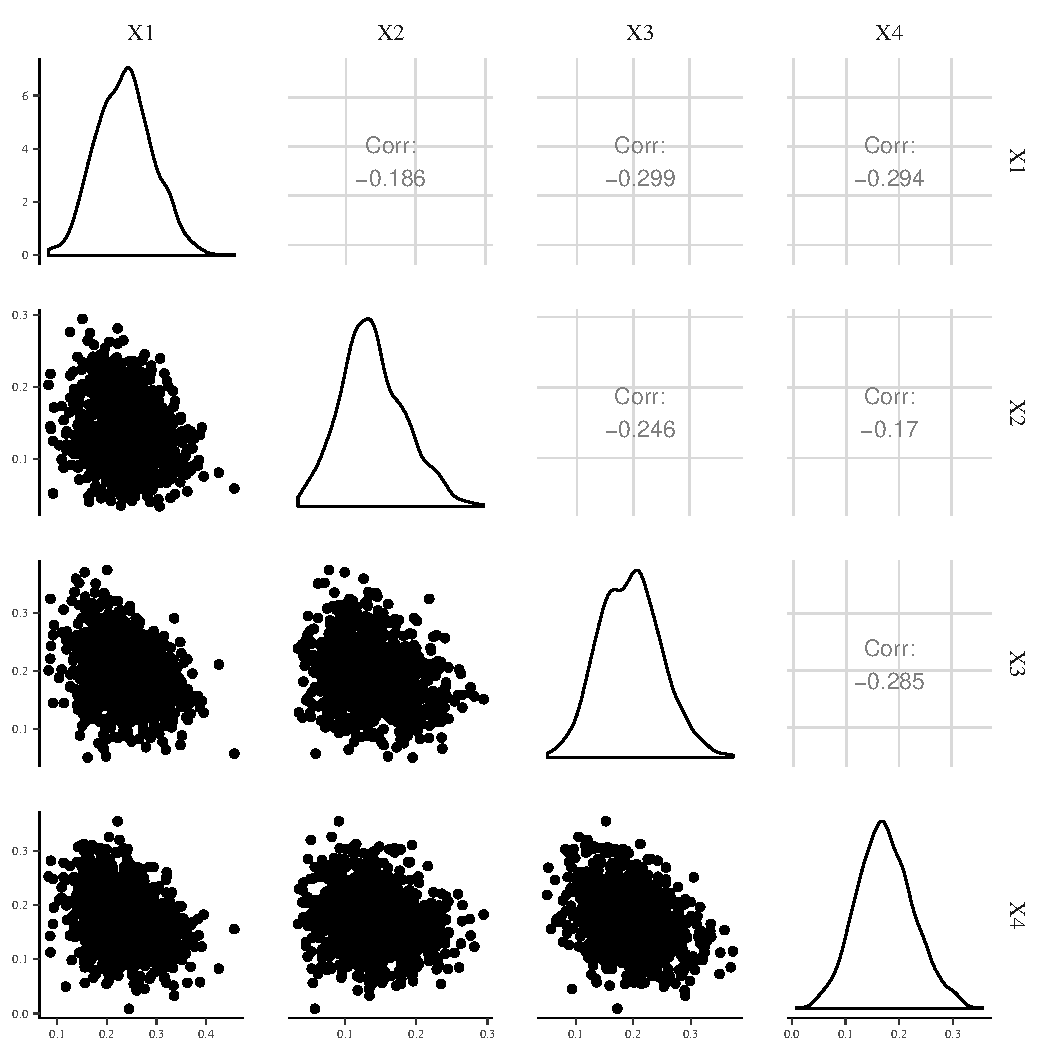
\includegraphics[width=\maxwidth]{figure/ch03_figsimdata_LMG-1} 
\begin{kframe}\begin{alltt}
\hlcom{# Comparison to relaimpo package}

\hlstd{fit} \hlkwb{<-} \hlkwd{lm}\hlstd{(y}\hlopt{~}\hlstd{.,} \hlkwc{data}\hlstd{=df)}

\hlcom{######## compare to relimp package}

\hlstd{run}\hlkwb{<-}\hlkwd{boot.relimp}\hlstd{(fit,} \hlkwc{fixed}\hlstd{=}\hlnum{TRUE}\hlstd{)}

\hlkwd{booteval.relimp}\hlstd{(run,} \hlkwc{bty} \hlstd{=} \hlstr{"perc"}\hlstd{,} \hlkwc{level} \hlstd{=} \hlnum{0.95}\hlstd{,}
                \hlkwc{sort} \hlstd{=} \hlnum{FALSE}\hlstd{,} \hlkwc{norank} \hlstd{=} \hlnum{TRUE}\hlstd{,} \hlkwc{nodiff} \hlstd{=} \hlnum{TRUE}\hlstd{,}
                \hlkwc{typesel} \hlstd{=} \hlkwd{c}\hlstd{(}\hlstr{"lmg"}\hlstd{))}
\end{alltt}
\begin{verbatim}
## Response variable: y 
## Total response variance: 5.552254 
## Analysis based on 50 observations 
## 
## 4 Regressors: 
## x1 x2 x3 x4 
## Proportion of variance explained by model: 82.41%
## Metrics are not normalized (rela=FALSE). 
## 
## Relative importance metrics: 
## 
##          lmg
## x1 0.1811296
## x2 0.1666997
## x3 0.3132778
## x4 0.1629547
## 
## Average coefficients for different model sizes: 
## 
##          1X       2Xs       3Xs       4Xs
## x1 1.074823 1.0625800 1.0486902 1.0286499
## x2 1.013182 0.9951801 0.9758422 0.9506321
## x3 1.293776 1.3391547 1.3728345 1.3889366
## x4 1.250949 1.1850119 1.0992265 0.9949324
## 
##  
##  Confidence interval information ( 1000 bootstrap replicates, bty= perc ): 
## Relative Contributions with confidence intervals: 
##  
##                   Lower  Upper
##        percentage 0.95   0.95  
## x1.lmg 0.1811     0.1009 0.2782
## x2.lmg 0.1667     0.0922 0.2607
## x3.lmg 0.3133     0.2169 0.4317
## x4.lmg 0.1630     0.0949 0.2506
## 
## CAUTION: Bootstrap confidence intervals can be somewhat liberal. 
## NOTE: X-matrix has been considered as fixed for bootstrapping.
\end{verbatim}
\end{kframe}
\end{knitrout}


Using the default uninformative priors, the LMG distributions obtained from the Bayesian framework are very similar to the bootstrap confidence intervals of the LMG estimates obtained from the relaimpo package. In both cases fixed regressors are assumed. In the example above the predictors were sampled from a normal distribution. It would therefore be more reasonable to assume stochastic predictors. As noted in ... under the assumption of weak exogeinity and conditional independence the posterior distributions of the regression paramters $\bbeta$ are valid for fixed and stochastic predictors. Inference about the covariance matrix can be seen as an independent problem. G recommends in most cases to use the non fixed regressor option when calculating bootstrap confidence intervals. The confidence intervals will then in general be a bit larger. If we want to include this uncertainty in the Bayesian framework, we would need some ideas about the distribution of the predictor variables $\X$. It is then possible to obtain poserior distributions of their corresponding covariance matrix. As a practical solution nonparametric bootstrap may be used to include the uncertainty of the covariance matrix. The following code includes the uncertainty of the stochastic predictors. 


\begin{knitrout}
\definecolor{shadecolor}{rgb}{0.969, 0.969, 0.969}\color{fgcolor}\begin{kframe}
\begin{alltt}
\hlcom{#Code assuming stochastic predictors}
\hlstd{run.stochastic}\hlkwb{<-}\hlkwd{boot.relimp}\hlstd{(fit,} \hlkwc{fixed}\hlstd{=}\hlnum{FALSE}\hlstd{)}

\hlkwd{booteval.relimp}\hlstd{(run.stochastic,} \hlkwc{bty} \hlstd{=} \hlstr{"perc"}\hlstd{,} \hlkwc{level} \hlstd{=} \hlnum{0.95}\hlstd{,}
                \hlkwc{sort} \hlstd{=} \hlnum{FALSE}\hlstd{,} \hlkwc{norank} \hlstd{=} \hlnum{TRUE}\hlstd{,} \hlkwc{nodiff} \hlstd{=} \hlnum{TRUE}\hlstd{,}
                \hlkwc{typesel} \hlstd{=} \hlkwd{c}\hlstd{(}\hlstr{"lmg"}\hlstd{))}
\end{alltt}
\begin{verbatim}
## Response variable: y 
## Total response variance: 5.552254 
## Analysis based on 50 observations 
## 
## 4 Regressors: 
## x1 x2 x3 x4 
## Proportion of variance explained by model: 82.41%
## Metrics are not normalized (rela=FALSE). 
## 
## Relative importance metrics: 
## 
##          lmg
## x1 0.1811296
## x2 0.1666997
## x3 0.3132778
## x4 0.1629547
## 
## Average coefficients for different model sizes: 
## 
##          1X       2Xs       3Xs       4Xs
## x1 1.074823 1.0625800 1.0486902 1.0286499
## x2 1.013182 0.9951801 0.9758422 0.9506321
## x3 1.293776 1.3391547 1.3728345 1.3889366
## x4 1.250949 1.1850119 1.0992265 0.9949324
## 
##  
##  Confidence interval information ( 1000 bootstrap replicates, bty= perc ): 
## Relative Contributions with confidence intervals: 
##  
##                   Lower  Upper
##        percentage 0.95   0.95  
## x1.lmg 0.1811     0.0784 0.3107
## x2.lmg 0.1667     0.0579 0.2927
## x3.lmg 0.3133     0.1648 0.4536
## x4.lmg 0.1630     0.0567 0.3131
## 
## CAUTION: Bootstrap confidence intervals can be somewhat liberal.
\end{verbatim}
\begin{alltt}
\hlcom{#----------------------------------------------------------------------------------------}


\hlstd{df.rtwos.boot} \hlkwb{<-}\hlkwd{rtwos.boot}\hlstd{(df[,}\hlnum{2}\hlopt{:}\hlnum{5}\hlstd{], post.sample,} \hlnum{10}\hlstd{)}

\hlstd{n.boot} \hlkwb{=} \hlnum{10}

\hlstd{LMG.Vals.boot}\hlkwb{<-}\hlkwd{array}\hlstd{(}\hlnum{0}\hlstd{,} \hlkwd{c}\hlstd{(}\hlnum{4}\hlstd{,}\hlkwd{dim}\hlstd{(df.rtwos.boot)[}\hlnum{2}\hlstd{], n.boot))}

\hlkwa{for} \hlstd{(b} \hlkwa{in} \hlnum{1}\hlopt{:}\hlstd{n.boot)\{}

\hlkwa{for}\hlstd{(i} \hlkwa{in} \hlnum{1}\hlopt{:}\hlkwd{dim}\hlstd{(df.rtwos.boot)[}\hlnum{2}\hlstd{])\{}

        \hlstd{gofn}\hlkwb{<-}\hlstd{df.rtwos.boot[,i,b]}

        \hlstd{obj.Gelman}\hlkwb{<-}\hlkwd{partition}\hlstd{(gofn,} \hlkwc{pcan} \hlstd{=} \hlnum{4}\hlstd{,} \hlkwc{var.names} \hlstd{=} \hlkwd{names}\hlstd{(df[,}\hlnum{2}\hlopt{:}\hlnum{5}\hlstd{]))}

        \hlstd{LMG.Vals.boot[,i, b]}\hlkwb{=}\hlstd{obj.Gelman}\hlopt{$}\hlstd{IJ[,}\hlnum{1}\hlstd{]}
\hlstd{\}}

\hlstd{\}}

\hlkwd{quantile}\hlstd{(}\hlkwd{c}\hlstd{(LMG.Vals.boot[}\hlnum{1}\hlstd{,}\hlnum{1}\hlopt{:}\hlnum{1000}\hlstd{,]),} \hlkwd{c}\hlstd{(}\hlnum{0.025}\hlstd{,} \hlnum{0.5}\hlstd{,} \hlnum{0.975}\hlstd{))}
\end{alltt}
\begin{verbatim}
##      2.5%       50%     97.5% 
## 0.0563607 0.1407858 0.2943099
\end{verbatim}
\begin{alltt}
\hlkwd{quantile}\hlstd{(}\hlkwd{c}\hlstd{(LMG.Vals.boot[}\hlnum{2}\hlstd{,}\hlnum{1}\hlopt{:}\hlnum{1000}\hlstd{,]),} \hlkwd{c}\hlstd{(}\hlnum{0.025}\hlstd{,} \hlnum{0.5}\hlstd{,} \hlnum{0.975}\hlstd{))}
\end{alltt}
\begin{verbatim}
##      2.5%       50%     97.5% 
## 0.0758204 0.1941894 0.3464876
\end{verbatim}
\begin{alltt}
\hlkwd{quantile}\hlstd{(}\hlkwd{c}\hlstd{(LMG.Vals.boot[}\hlnum{3}\hlstd{,}\hlnum{1}\hlopt{:}\hlnum{1000}\hlstd{,]),} \hlkwd{c}\hlstd{(}\hlnum{0.025}\hlstd{,} \hlnum{0.5}\hlstd{,} \hlnum{0.975}\hlstd{))}
\end{alltt}
\begin{verbatim}
##      2.5%       50%     97.5% 
## 0.1151979 0.2832940 0.4079618
\end{verbatim}
\begin{alltt}
\hlkwd{quantile}\hlstd{(}\hlkwd{c}\hlstd{(LMG.Vals.boot[}\hlnum{4}\hlstd{,}\hlnum{1}\hlopt{:}\hlnum{1000}\hlstd{,]),} \hlkwd{c}\hlstd{(}\hlnum{0.025}\hlstd{,} \hlnum{0.5}\hlstd{,} \hlnum{0.975}\hlstd{))}
\end{alltt}
\begin{verbatim}
##       2.5%        50%      97.5% 
## 0.04244554 0.16971870 0.31231758
\end{verbatim}
\begin{alltt}
\hlcom{#very similar values as in the confidence intervals for stochastic predictors}


\hlcom{#what if we have prior knowledge}
\hlstd{my_prior} \hlkwb{<-} \hlkwd{normal}\hlstd{(}\hlkwc{location} \hlstd{=} \hlkwd{c}\hlstd{(}\hlnum{1}\hlstd{,} \hlnum{1}\hlstd{,}\hlnum{1}\hlstd{,}\hlnum{1}\hlstd{),} \hlkwc{scale} \hlstd{=} \hlkwd{c}\hlstd{(}\hlnum{0.01}\hlstd{,} \hlnum{0.01}\hlstd{,}\hlnum{0.01}\hlstd{,}\hlnum{0.01}\hlstd{),} \hlkwc{autoscale} \hlstd{=} \hlnum{FALSE}\hlstd{)}

\hlstd{post2} \hlkwb{<-} \hlkwd{stan_glm}\hlstd{(y} \hlopt{~} \hlnum{1} \hlopt{+} \hlstd{x1} \hlopt{+} \hlstd{x2} \hlopt{+} \hlstd{x3} \hlopt{+} \hlstd{x4,}
                  \hlkwc{data} \hlstd{= df,} \hlkwc{prior} \hlstd{= my_prior,}
                  \hlkwc{chains} \hlstd{=} \hlnum{2}\hlstd{,} \hlkwc{cores} \hlstd{=} \hlnum{1}\hlstd{)}
\end{alltt}
\begin{verbatim}
## 
## SAMPLING FOR MODEL 'continuous' NOW (CHAIN 1).
## 
## Gradient evaluation took 0.000117 seconds
## 1000 transitions using 10 leapfrog steps per transition would take 1.17 seconds.
## Adjust your expectations accordingly!
## 
## 
## Iteration:    1 / 2000 [  0%]  (Warmup)
## Iteration:  200 / 2000 [ 10%]  (Warmup)
## Iteration:  400 / 2000 [ 20%]  (Warmup)
## Iteration:  600 / 2000 [ 30%]  (Warmup)
## Iteration:  800 / 2000 [ 40%]  (Warmup)
## Iteration: 1000 / 2000 [ 50%]  (Warmup)
## Iteration: 1001 / 2000 [ 50%]  (Sampling)
## Iteration: 1200 / 2000 [ 60%]  (Sampling)
## Iteration: 1400 / 2000 [ 70%]  (Sampling)
## Iteration: 1600 / 2000 [ 80%]  (Sampling)
## Iteration: 1800 / 2000 [ 90%]  (Sampling)
## Iteration: 2000 / 2000 [100%]  (Sampling)
## 
##  Elapsed Time: 0.08434 seconds (Warm-up)
##                0.062999 seconds (Sampling)
##                0.147339 seconds (Total)
## 
## 
## SAMPLING FOR MODEL 'continuous' NOW (CHAIN 2).
## 
## Gradient evaluation took 1.6e-05 seconds
## 1000 transitions using 10 leapfrog steps per transition would take 0.16 seconds.
## Adjust your expectations accordingly!
## 
## 
## Iteration:    1 / 2000 [  0%]  (Warmup)
## Iteration:  200 / 2000 [ 10%]  (Warmup)
## Iteration:  400 / 2000 [ 20%]  (Warmup)
## Iteration:  600 / 2000 [ 30%]  (Warmup)
## Iteration:  800 / 2000 [ 40%]  (Warmup)
## Iteration: 1000 / 2000 [ 50%]  (Warmup)
## Iteration: 1001 / 2000 [ 50%]  (Sampling)
## Iteration: 1200 / 2000 [ 60%]  (Sampling)
## Iteration: 1400 / 2000 [ 70%]  (Sampling)
## Iteration: 1600 / 2000 [ 80%]  (Sampling)
## Iteration: 1800 / 2000 [ 90%]  (Sampling)
## Iteration: 2000 / 2000 [100%]  (Sampling)
## 
##  Elapsed Time: 0.103181 seconds (Warm-up)
##                0.063035 seconds (Sampling)
##                0.166216 seconds (Total)
\end{verbatim}
\begin{alltt}
\hlcom{#posterior sample}
\hlstd{post.sample} \hlkwb{<-} \hlkwd{as.matrix}\hlstd{(post2)}

\hlcom{#example of the first 10 posterior samples}
\hlstd{post.sample[}\hlnum{1}\hlopt{:}\hlnum{10}\hlstd{,]}
\end{alltt}
\begin{verbatim}
##           parameters
## iterations (Intercept)        x1        x2        x3        x4     sigma
##       [1,]  0.20013187 0.9951292 0.9836621 0.9862314 0.9920344 1.0069258
##       [2,] -0.17301698 1.0027072 1.0099915 1.0217840 0.9964729 1.1497936
##       [3,]  0.26606459 1.0002421 0.9906716 0.9853976 1.0025311 1.1194660
##       [4,]  0.23934385 0.9913646 1.0054863 0.9887745 0.9994093 0.9760771
##       [5,]  0.10217015 0.9917333 1.0084500 0.9925039 0.9939052 0.9815683
##       [6,] -0.17613916 1.0034315 1.0090995 1.0053460 0.9811486 1.0075087
##       [7,]  0.01952345 0.9996066 0.9969790 1.0070605 0.9794494 0.9698949
##       [8,]  0.10767092 1.0006765 1.0017746 1.0014465 1.0108357 1.1981013
##       [9,] -0.20811507 1.0081525 1.0074328 0.9894853 0.9867378 1.0760004
##      [10,]  0.09935476 1.0115203 0.9977477 1.0142334 0.9973044 1.0099387
\end{verbatim}
\begin{alltt}
\hlcom{#no need for the intercept, last parameter is sigma}
\hlstd{post.sample} \hlkwb{<-} \hlstd{post.sample[,}\hlopt{-}\hlnum{1}\hlstd{]}


\hlcom{#data frame with all submodels}


\hlstd{df.rtwos.boot} \hlkwb{<-}\hlkwd{rtwos.boot}\hlstd{(df[,}\hlnum{2}\hlopt{:}\hlnum{5}\hlstd{], post.sample,} \hlnum{10}\hlstd{)}

\hlstd{n.boot} \hlkwb{=} \hlnum{10}

\hlstd{LMG.Vals.boot}\hlkwb{<-}\hlkwd{array}\hlstd{(}\hlnum{0}\hlstd{,} \hlkwd{c}\hlstd{(}\hlnum{4}\hlstd{,}\hlkwd{dim}\hlstd{(df.rtwos.boot)[}\hlnum{2}\hlstd{], n.boot))}

\hlkwa{for} \hlstd{(b} \hlkwa{in} \hlnum{1}\hlopt{:}\hlstd{n.boot)\{}

\hlkwa{for}\hlstd{(i} \hlkwa{in} \hlnum{1}\hlopt{:}\hlkwd{dim}\hlstd{(df.rtwos.boot)[}\hlnum{2}\hlstd{])\{}

        \hlstd{gofn}\hlkwb{<-}\hlstd{df.rtwos.boot[,i,b]}

        \hlstd{obj.Gelman}\hlkwb{<-}\hlkwd{partition}\hlstd{(gofn,} \hlkwc{pcan} \hlstd{=} \hlnum{4}\hlstd{,} \hlkwc{var.names} \hlstd{=} \hlkwd{names}\hlstd{(df[,}\hlnum{2}\hlopt{:}\hlnum{5}\hlstd{]))}

        \hlstd{LMG.Vals.boot[,i, b]}\hlkwb{=}\hlstd{obj.Gelman}\hlopt{$}\hlstd{IJ[,}\hlnum{1}\hlstd{]}
\hlstd{\}}

\hlstd{\}}

\hlkwd{quantile}\hlstd{(}\hlkwd{c}\hlstd{(LMG.Vals.boot[}\hlnum{1}\hlstd{,}\hlnum{1}\hlopt{:}\hlnum{1000}\hlstd{,]),} \hlkwd{c}\hlstd{(}\hlnum{0.025}\hlstd{,} \hlnum{0.5}\hlstd{,} \hlnum{0.975}\hlstd{))}
\end{alltt}
\begin{verbatim}
##      2.5%       50%     97.5% 
## 0.1381109 0.2030829 0.3103296
\end{verbatim}
\begin{alltt}
\hlkwd{quantile}\hlstd{(}\hlkwd{c}\hlstd{(LMG.Vals.boot[}\hlnum{2}\hlstd{,}\hlnum{1}\hlopt{:}\hlnum{1000}\hlstd{,]),} \hlkwd{c}\hlstd{(}\hlnum{0.025}\hlstd{,} \hlnum{0.5}\hlstd{,} \hlnum{0.975}\hlstd{))}
\end{alltt}
\begin{verbatim}
##      2.5%       50%     97.5% 
## 0.1497110 0.1935097 0.2664145
\end{verbatim}
\begin{alltt}
\hlkwd{quantile}\hlstd{(}\hlkwd{c}\hlstd{(LMG.Vals.boot[}\hlnum{3}\hlstd{,}\hlnum{1}\hlopt{:}\hlnum{1000}\hlstd{,]),} \hlkwd{c}\hlstd{(}\hlnum{0.025}\hlstd{,} \hlnum{0.5}\hlstd{,} \hlnum{0.975}\hlstd{))}
\end{alltt}
\begin{verbatim}
##      2.5%       50%     97.5% 
## 0.1015362 0.1829171 0.2721100
\end{verbatim}
\begin{alltt}
\hlkwd{quantile}\hlstd{(}\hlkwd{c}\hlstd{(LMG.Vals.boot[}\hlnum{4}\hlstd{,}\hlnum{1}\hlopt{:}\hlnum{1000}\hlstd{,]),} \hlkwd{c}\hlstd{(}\hlnum{0.025}\hlstd{,} \hlnum{0.5}\hlstd{,} \hlnum{0.975}\hlstd{))}
\end{alltt}
\begin{verbatim}
##       2.5%        50%      97.5% 
## 0.06347948 0.16874963 0.24271955
\end{verbatim}
\end{kframe}
\end{knitrout}

In the following example we know that the $\X$ are coming from a normal distribution. The covariance matrix of the distribution is estimated in a Bayesian way. The package Jags is used.

\begin{knitrout}
\definecolor{shadecolor}{rgb}{0.969, 0.969, 0.969}\color{fgcolor}\begin{kframe}
\begin{alltt}
\hlstd{zy} \hlkwb{=} \hlstd{df[,}\hlnum{2}\hlopt{:}\hlnum{5}\hlstd{]}

\hlcom{#----------------------------------------------------------------------------}
\hlcom{# The rest can remain unchanged, except for the specification of difference of}
\hlcom{# correlations at the very end.}
\hlcom{#----------------------------------------------------------------------------}

\hlcom{# Load some functions used below:}
\hlcom{# Install the ellipse package if not already:}
\hlcom{# Standardize the data:}

\hlcom{#zy = apply(y,2,function(yVec)\{(yVec-mean(yVec))/sd(yVec)\})}
\hlcom{# Assemble data for sending to JAGS:}
\hlstd{dataList} \hlkwb{=} \hlkwd{list}\hlstd{(}
        \hlkwc{zy} \hlstd{= zy ,}
        \hlkwc{Ntotal} \hlstd{=}  \hlkwd{nrow}\hlstd{(zy) ,}
        \hlkwc{Nvar} \hlstd{=} \hlkwd{ncol}\hlstd{(zy) ,}
        \hlcom{# Include original data info for transforming to original scale:}
        \hlcom{# For wishart (dwish) prior on inverse covariance matrix:}
        \hlkwc{zRscal} \hlstd{=} \hlkwd{ncol}\hlstd{(zy) ,}  \hlcom{# for dwish prior}
        \hlkwc{zRmat} \hlstd{=} \hlkwd{diag}\hlstd{(}\hlkwc{x}\hlstd{=}\hlnum{1}\hlstd{,}\hlkwc{nrow}\hlstd{=}\hlkwd{ncol}\hlstd{(zy))}  \hlcom{# Rmat = diag(apply(y,2,var))}
\hlstd{)}

\hlcom{# Define the model:}
\hlstd{modelString} \hlkwb{=} \hlstr{"
model \{
for ( i in 1:Ntotal ) \{
zy[i,1:Nvar] ~ dmnorm( zMu[1:Nvar] , zInvCovMat[1:Nvar,1:Nvar] ) 
\}
for ( varIdx in 1:Nvar ) \{ zMu[varIdx] ~ dnorm( 0 , 1/2^2 ) \}
zInvCovMat ~ dwish( zRmat[1:Nvar,1:Nvar] , zRscal )
# Convert invCovMat to sd and correlation:
zCovMat <- inverse( zInvCovMat )

\}
"} \hlcom{# close quote for modelString}
\hlkwd{writeLines}\hlstd{( modelString ,} \hlkwc{con}\hlstd{=}\hlstr{"Jags-MultivariateNormal-model.txt"} \hlstd{)}

\hlcom{# Run the chains:}
\hlstd{nChain} \hlkwb{=} \hlnum{3}
\hlstd{nAdapt} \hlkwb{=} \hlnum{500}
\hlstd{nBurnIn} \hlkwb{=} \hlnum{500}
\hlstd{nThin} \hlkwb{=} \hlnum{10}
\hlstd{nStepToSave} \hlkwb{=} \hlnum{20000}
\hlkwd{require}\hlstd{(rjags)}
\hlstd{jagsModel} \hlkwb{=} \hlkwd{jags.model}\hlstd{(} \hlkwc{file}\hlstd{=}\hlstr{"Jags-MultivariateNormal-model.txt"} \hlstd{,}
                                                                                                \hlkwc{data}\hlstd{=dataList ,} \hlkwc{n.chains}\hlstd{=nChain ,} \hlkwc{n.adapt}\hlstd{=nAdapt )}
\end{alltt}
\begin{verbatim}
## Compiling model graph
##    Resolving undeclared variables
##    Allocating nodes
## Graph information:
##    Observed stochastic nodes: 50
##    Unobserved stochastic nodes: 5
##    Total graph size: 82
## 
## Initializing model
\end{verbatim}
\begin{alltt}
\hlkwd{update}\hlstd{( jagsModel ,} \hlkwc{n.iter}\hlstd{=nBurnIn )}
\hlstd{codaSamples} \hlkwb{=} \hlkwd{coda.samples}\hlstd{( jagsModel ,}
                                                                                                                \hlkwc{variable.names}\hlstd{=}\hlkwd{c}\hlstd{(}\hlstr{'zCovMat'}\hlstd{) ,}
                                                                                                                \hlkwc{n.iter}\hlstd{=nStepToSave}\hlopt{/}\hlstd{nChain}\hlopt{*}\hlstd{nThin ,} \hlkwc{thin}\hlstd{=nThin )}


\hlcom{# Convergence diagnostics:}
\hlstd{parameterNames} \hlkwb{=} \hlkwd{varnames}\hlstd{(codaSamples)} \hlcom{# get all parameter names}


\hlcom{# Examine the posterior distribution:}
\hlstd{mcmcMat} \hlkwb{=} \hlkwd{as.matrix}\hlstd{(codaSamples)}
\hlstd{chainLength} \hlkwb{=} \hlkwd{nrow}\hlstd{(mcmcMat)}

\hlstd{covMat} \hlkwb{<-} \hlkwd{array}\hlstd{(}\hlnum{NA}\hlstd{,} \hlkwd{c}\hlstd{(}\hlnum{4}\hlstd{,}\hlnum{4}\hlstd{,chainLength))}

\hlkwa{for} \hlstd{(i} \hlkwa{in} \hlnum{1}\hlopt{:}\hlstd{chainLength)\{}
\hlstd{covMat[}\hlnum{1}\hlopt{:}\hlnum{4}\hlstd{,}\hlnum{1}\hlopt{:}\hlnum{4}\hlstd{,i]}\hlkwb{<-}\hlkwd{matrix}\hlstd{(mcmcMat[i,],} \hlnum{4}\hlstd{,} \hlnum{4}\hlstd{)}
\hlstd{\}}

\hlstd{covMat} \hlkwb{<-} \hlstd{covMat[}\hlnum{1}\hlopt{:}\hlnum{4}\hlstd{,}\hlnum{1}\hlopt{:}\hlnum{4}\hlstd{,}\hlkwd{sample}\hlstd{(}\hlnum{1}\hlopt{:}\hlnum{20000}\hlstd{,} \hlkwc{replace}\hlstd{=F)]}


\hlstd{df.rtwos} \hlkwb{<-}\hlkwd{rtwos.covm}\hlstd{(df[,}\hlnum{2}\hlopt{:}\hlnum{5}\hlstd{], post.sample, covMat,} \hlnum{10}\hlstd{)}


\hlstd{n.boot} \hlkwb{=} \hlnum{10}

\hlstd{LMG.Vals}\hlkwb{<-}\hlkwd{array}\hlstd{(}\hlnum{0}\hlstd{,} \hlkwd{c}\hlstd{(}\hlnum{4}\hlstd{,}\hlkwd{dim}\hlstd{(df.rtwos)[}\hlnum{2}\hlstd{], n.boot))}

\hlkwa{for} \hlstd{(b} \hlkwa{in} \hlnum{1}\hlopt{:}\hlstd{n.boot)\{}

        \hlkwa{for}\hlstd{(i} \hlkwa{in} \hlnum{1}\hlopt{:}\hlkwd{dim}\hlstd{(df.rtwos)[}\hlnum{2}\hlstd{])\{}

                \hlstd{gofn}\hlkwb{<-}\hlstd{df.rtwos[,i,b]}

                \hlstd{obj.Gelman}\hlkwb{<-}\hlkwd{partition}\hlstd{(gofn,} \hlkwc{pcan} \hlstd{=} \hlnum{4}\hlstd{,} \hlkwc{var.names} \hlstd{=} \hlkwd{names}\hlstd{(df[,}\hlnum{2}\hlopt{:}\hlnum{5}\hlstd{]))}

                \hlstd{LMG.Vals[,i, b]}\hlkwb{=}\hlstd{obj.Gelman}\hlopt{$}\hlstd{IJ[,}\hlnum{1}\hlstd{]}
        \hlstd{\}}

\hlstd{\}}

\hlkwd{quantile}\hlstd{(}\hlkwd{c}\hlstd{(LMG.Vals[}\hlnum{1}\hlstd{,}\hlnum{1}\hlopt{:}\hlnum{1000}\hlstd{,]),} \hlkwd{c}\hlstd{(}\hlnum{0.025}\hlstd{,} \hlnum{0.5}\hlstd{,} \hlnum{0.975}\hlstd{))}
\end{alltt}
\begin{verbatim}
##       2.5%        50%      97.5% 
## 0.07955934 0.19561327 0.25671047
\end{verbatim}
\begin{alltt}
\hlkwd{quantile}\hlstd{(}\hlkwd{c}\hlstd{(LMG.Vals[}\hlnum{2}\hlstd{,}\hlnum{1}\hlopt{:}\hlnum{1000}\hlstd{,]),} \hlkwd{c}\hlstd{(}\hlnum{0.025}\hlstd{,} \hlnum{0.5}\hlstd{,} \hlnum{0.975}\hlstd{))}
\end{alltt}
\begin{verbatim}
##      2.5%       50%     97.5% 
## 0.1059393 0.1921079 0.3129919
\end{verbatim}
\begin{alltt}
\hlkwd{quantile}\hlstd{(}\hlkwd{c}\hlstd{(LMG.Vals[}\hlnum{3}\hlstd{,}\hlnum{1}\hlopt{:}\hlnum{1000}\hlstd{,]),} \hlkwd{c}\hlstd{(}\hlnum{0.025}\hlstd{,} \hlnum{0.5}\hlstd{,} \hlnum{0.975}\hlstd{))}
\end{alltt}
\begin{verbatim}
##      2.5%       50%     97.5% 
## 0.1073336 0.1822257 0.2556199
\end{verbatim}
\begin{alltt}
\hlkwd{quantile}\hlstd{(}\hlkwd{c}\hlstd{(LMG.Vals[}\hlnum{4}\hlstd{,}\hlnum{1}\hlopt{:}\hlnum{1000}\hlstd{,]),} \hlkwd{c}\hlstd{(}\hlnum{0.025}\hlstd{,} \hlnum{0.5}\hlstd{,} \hlnum{0.975}\hlstd{))}
\end{alltt}
\begin{verbatim}
##      2.5%       50%     97.5% 
## 0.1192879 0.1863754 0.3401010
\end{verbatim}
\end{kframe}
\end{knitrout}

Using the bootstrap samples of the covariance matrix or samples from the posterior covariance matrix resulted in very similar LMG values. Bootstrap seems to be a valuable option for stochastic predictors when the distribution of the predictors is unknown. Even when the distribution is known the difference seems to be tiny. A benefit of going the full Bayesian way is that we can also include prior knowledge of the covariance matrix. For stochastic predictors the uncertainty about the covariance matrix is reflected in the large credible intervals. Even when we would knew the exact regression parameters, there is alot of uncertainty in the LMG values caused by the uncertainty about the covariance matrix. Code xx shows the uncertainty about the LMG values caused by the uncertainty about the covariance matrix. 

Another interesting option in some cases would be to use the shrinkage estimate of the covariance matrix. 


\begin{knitrout}
\definecolor{shadecolor}{rgb}{0.969, 0.969, 0.969}\color{fgcolor}\begin{kframe}
\begin{alltt}
\hlcom{#How much variance is effectively in the bootstrap matrix when we know the regression parameters.}

\hlcom{#fake post sample}

\hlstd{x1} \hlkwb{<-} \hlkwd{rnorm}\hlstd{(}\hlnum{50}\hlstd{,} \hlnum{0}\hlstd{,} \hlnum{1}\hlstd{); x2} \hlkwb{<-} \hlkwd{rnorm}\hlstd{(}\hlnum{50}\hlstd{,} \hlnum{0}\hlstd{,} \hlnum{1}\hlstd{)}
\hlstd{x3} \hlkwb{<-} \hlkwd{rnorm}\hlstd{(}\hlnum{50}\hlstd{,} \hlnum{0}\hlstd{,} \hlnum{1}\hlstd{); x4} \hlkwb{<-} \hlkwd{rnorm}\hlstd{(}\hlnum{50}\hlstd{,} \hlnum{0}\hlstd{,} \hlnum{1}\hlstd{)}
\hlcom{#b1 <- 0.5; b2 <- 1; b3 <- 2; b4 <- 0}
\hlstd{b1} \hlkwb{<-} \hlnum{1}\hlstd{; b2} \hlkwb{<-} \hlnum{1}\hlstd{; b3} \hlkwb{<-} \hlnum{1}\hlstd{; b4} \hlkwb{<-} \hlnum{1}

\hlstd{y} \hlkwb{<-} \hlstd{b1}\hlopt{*}\hlstd{x1} \hlopt{+} \hlstd{x2}\hlopt{*}\hlstd{b2} \hlopt{+} \hlstd{b3}\hlopt{*}\hlstd{x3} \hlopt{+} \hlstd{b4}\hlopt{*}\hlstd{x4} \hlopt{+} \hlkwd{rnorm}\hlstd{(}\hlnum{50}\hlstd{,} \hlnum{0}\hlstd{,} \hlnum{1}\hlstd{)}

\hlstd{df} \hlkwb{<-} \hlkwd{data.frame}\hlstd{(}\hlkwc{y} \hlstd{= y,} \hlkwc{x1} \hlstd{= x1,} \hlkwc{x2} \hlstd{= x2,} \hlkwc{x3} \hlstd{= x3,} \hlkwc{x4} \hlstd{= x4)}

\hlstd{post.sample} \hlkwb{<-} \hlkwd{matrix}\hlstd{(}\hlnum{1}\hlstd{,} \hlnum{1}\hlstd{,}\hlnum{5}\hlstd{)}

\hlstd{df.rtwos.boot} \hlkwb{<-}\hlkwd{rtwos.boot}\hlstd{(df[,}\hlnum{2}\hlopt{:}\hlnum{5}\hlstd{], post.sample,} \hlnum{1000}\hlstd{)}

\hlstd{n.boot} \hlkwb{=} \hlnum{1000}

\hlstd{LMG.Vals.boot}\hlkwb{<-}\hlkwd{array}\hlstd{(}\hlnum{0}\hlstd{,} \hlkwd{c}\hlstd{(}\hlnum{4}\hlstd{,}\hlkwd{dim}\hlstd{(df.rtwos.boot)[}\hlnum{2}\hlstd{], n.boot))}

\hlkwa{for} \hlstd{(b} \hlkwa{in} \hlnum{1}\hlopt{:}\hlstd{n.boot)\{}

\hlkwa{for}\hlstd{(i} \hlkwa{in} \hlnum{1}\hlopt{:}\hlkwd{dim}\hlstd{(df.rtwos.boot)[}\hlnum{2}\hlstd{])\{}

        \hlstd{gofn}\hlkwb{<-}\hlstd{df.rtwos.boot[,i,b]}

        \hlstd{obj.Gelman}\hlkwb{<-}\hlkwd{partition}\hlstd{(gofn,} \hlkwc{pcan} \hlstd{=} \hlnum{4}\hlstd{,} \hlkwc{var.names} \hlstd{=} \hlkwd{names}\hlstd{(df[,}\hlnum{2}\hlopt{:}\hlnum{5}\hlstd{]))}

        \hlstd{LMG.Vals.boot[,i, b]}\hlkwb{=}\hlstd{obj.Gelman}\hlopt{$}\hlstd{IJ[,}\hlnum{1}\hlstd{]}
\hlstd{\}}

\hlstd{\}}

\hlkwd{quantile}\hlstd{(}\hlkwd{c}\hlstd{(LMG.Vals.boot[}\hlnum{1}\hlstd{,}\hlnum{1}\hlstd{,]),} \hlkwd{c}\hlstd{(}\hlnum{0.025}\hlstd{,} \hlnum{0.5}\hlstd{,} \hlnum{0.975}\hlstd{))}
\end{alltt}
\begin{verbatim}
##      2.5%       50%     97.5% 
## 0.0979818 0.1894039 0.2799671
\end{verbatim}
\begin{alltt}
\hlkwd{quantile}\hlstd{(}\hlkwd{c}\hlstd{(LMG.Vals.boot[}\hlnum{2}\hlstd{,}\hlnum{1}\hlstd{,]),} \hlkwd{c}\hlstd{(}\hlnum{0.025}\hlstd{,} \hlnum{0.5}\hlstd{,} \hlnum{0.975}\hlstd{))}
\end{alltt}
\begin{verbatim}
##      2.5%       50%     97.5% 
## 0.1773573 0.2536383 0.3293491
\end{verbatim}
\begin{alltt}
\hlkwd{quantile}\hlstd{(}\hlkwd{c}\hlstd{(LMG.Vals.boot[}\hlnum{3}\hlstd{,}\hlnum{1}\hlstd{,]),} \hlkwd{c}\hlstd{(}\hlnum{0.025}\hlstd{,} \hlnum{0.5}\hlstd{,} \hlnum{0.975}\hlstd{))}
\end{alltt}
\begin{verbatim}
##       2.5%        50%      97.5% 
## 0.07376485 0.13427948 0.21775383
\end{verbatim}
\begin{alltt}
\hlkwd{quantile}\hlstd{(}\hlkwd{c}\hlstd{(LMG.Vals.boot[}\hlnum{4}\hlstd{,}\hlnum{1}\hlstd{,]),} \hlkwd{c}\hlstd{(}\hlnum{0.025}\hlstd{,} \hlnum{0.5}\hlstd{,} \hlnum{0.975}\hlstd{))}
\end{alltt}
\begin{verbatim}
##      2.5%       50%     97.5% 
## 0.1266168 0.1955925 0.2684755
\end{verbatim}
\begin{alltt}
\hlstd{dat} \hlkwb{<-} \hlkwd{data.frame}\hlstd{(}\hlkwd{t}\hlstd{(LMG.Vals.boot[}\hlnum{1}\hlopt{:}\hlnum{4}\hlstd{,}\hlnum{1}\hlstd{,]))}
\hlstd{pairs.chart} \hlkwb{<-} \hlkwd{ggpairs}\hlstd{(dat,} \hlkwc{lower} \hlstd{=} \hlkwd{list}\hlstd{(}\hlkwd{list}\hlstd{(}\hlkwc{combo} \hlstd{=} \hlstr{"facetdensity"}\hlstd{)),} \hlkwc{upper} \hlstd{=} \hlkwd{list}\hlstd{(}\hlkwd{list}\hlstd{(}\hlkwc{continuous} \hlstd{=} \hlstr{"cor"}\hlstd{)))} \hlopt{+} \hlstd{ggplot2}\hlopt{::}\hlkwd{theme}\hlstd{(}\hlkwc{axis.text} \hlstd{=} \hlkwd{element_text}\hlstd{(}\hlkwc{size} \hlstd{=} \hlnum{6}\hlstd{))}
\hlstd{pairs.chart}
\end{alltt}
\end{kframe}
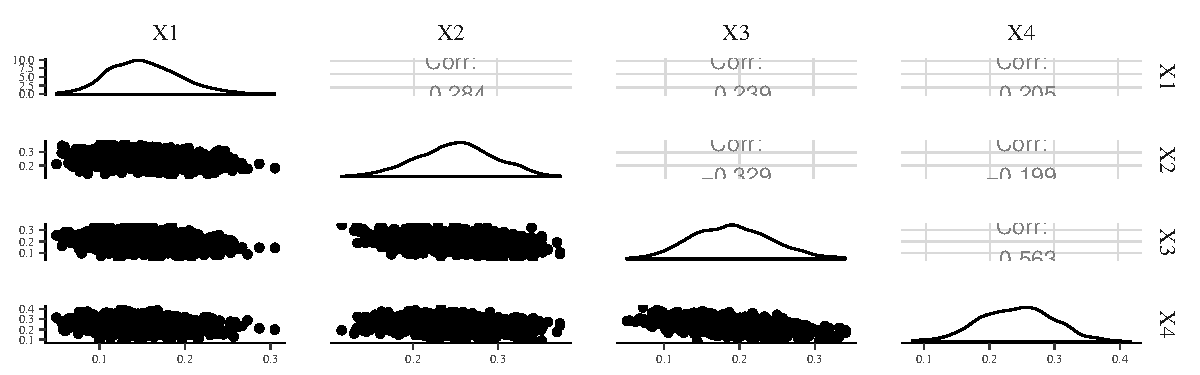
\includegraphics[width=\maxwidth]{figure/ch03_figcovuncertainty-1} 
\begin{kframe}\begin{alltt}
\hlkwd{cov}\hlstd{(df[,}\hlnum{2}\hlopt{:}\hlnum{5}\hlstd{])}
\end{alltt}
\begin{verbatim}
##            x1         x2          x3          x4
## x1  0.8507778  0.2803422 -0.10769517 -0.10821297
## x2  0.2803422  1.0379131 -0.16375752  0.06331260
## x3 -0.1076952 -0.1637575  0.80799891  0.05999761
## x4 -0.1082130  0.0633126  0.05999761  0.89839912
\end{verbatim}
\end{kframe}
\end{knitrout}

\begin{knitrout}
\definecolor{shadecolor}{rgb}{0.969, 0.969, 0.969}\color{fgcolor}\begin{kframe}
\begin{alltt}
\hlcom{#Comparison of sample covariance and shrink covariance matrix}

\hlkwd{cov}\hlstd{(df[,}\hlnum{2}\hlopt{:}\hlnum{5}\hlstd{])}
\end{alltt}
\begin{verbatim}
##              x1          x2           x3         x4
## x1  0.918802371 -0.10264450  0.009003572  0.1281456
## x2 -0.102644497  0.97559948 -0.012534282  0.1849557
## x3  0.009003572 -0.01253428  0.961040604 -0.0892520
## x4  0.128145565  0.18495569 -0.089252004  0.7174392
\end{verbatim}
\begin{alltt}
\hlkwd{cov.shrink}\hlstd{(df[,}\hlnum{2}\hlopt{:}\hlnum{5}\hlstd{])}
\end{alltt}
\begin{verbatim}
## Estimating optimal shrinkage intensity lambda.var (variance vector): 1 
## 
## Estimating optimal shrinkage intensity lambda (correlation matrix): 1
##           x1        x2        x3        x4
## x1 0.9399215 0.0000000 0.0000000 0.0000000
## x2 0.0000000 0.9399215 0.0000000 0.0000000
## x3 0.0000000 0.0000000 0.9399215 0.0000000
## x4 0.0000000 0.0000000 0.0000000 0.9399215
## attr(,"lambda")
## [1] 1
## attr(,"lambda.estimated")
## [1] TRUE
## attr(,"class")
## [1] "shrinkage"
## attr(,"lambda.var")
## [1] 1
## attr(,"lambda.var.estimated")
## [1] TRUE
\end{verbatim}
\end{kframe}
\end{knitrout}

\section{Real World Data}


The following example data are taken from the book Bayesian Regression Modeling with INLA. The data were about air pollution in 41 cities in the United States originally published in Everitt (2006). The data consits of the SO2 level as the dependent variable and six explanatory variables 
Two of the explanatory variables are are related to human ecology (pop, manuf) and four others are related to climate (negtemp, wind, precip, days).


\begin{table}
\caption{Variable description of air pollution data}
\begin{tabularx}{\textwidth}{|l|X|l|}
  \hline			
  Variable Name & Description & Codes/Values \\   \hline  
  SO2 & sulfur dioxide content of air & microgrames per cubic meter \\
  negtemp & negative value of average & fahrenheit\\
  manuf & number of manufacturing enterprises employing 20 or more workers & integers \\
  pop & population size in thousands (1970 census) & numbers \\
  wind & average wind speed & miles per hour \\
  precip & average annual percipitation & inches \\
  days & average munber of days with precipitation per year & integers \\
  \hline  
\end{tabularx}
\label{table:airpollutiondata}
\end{table}


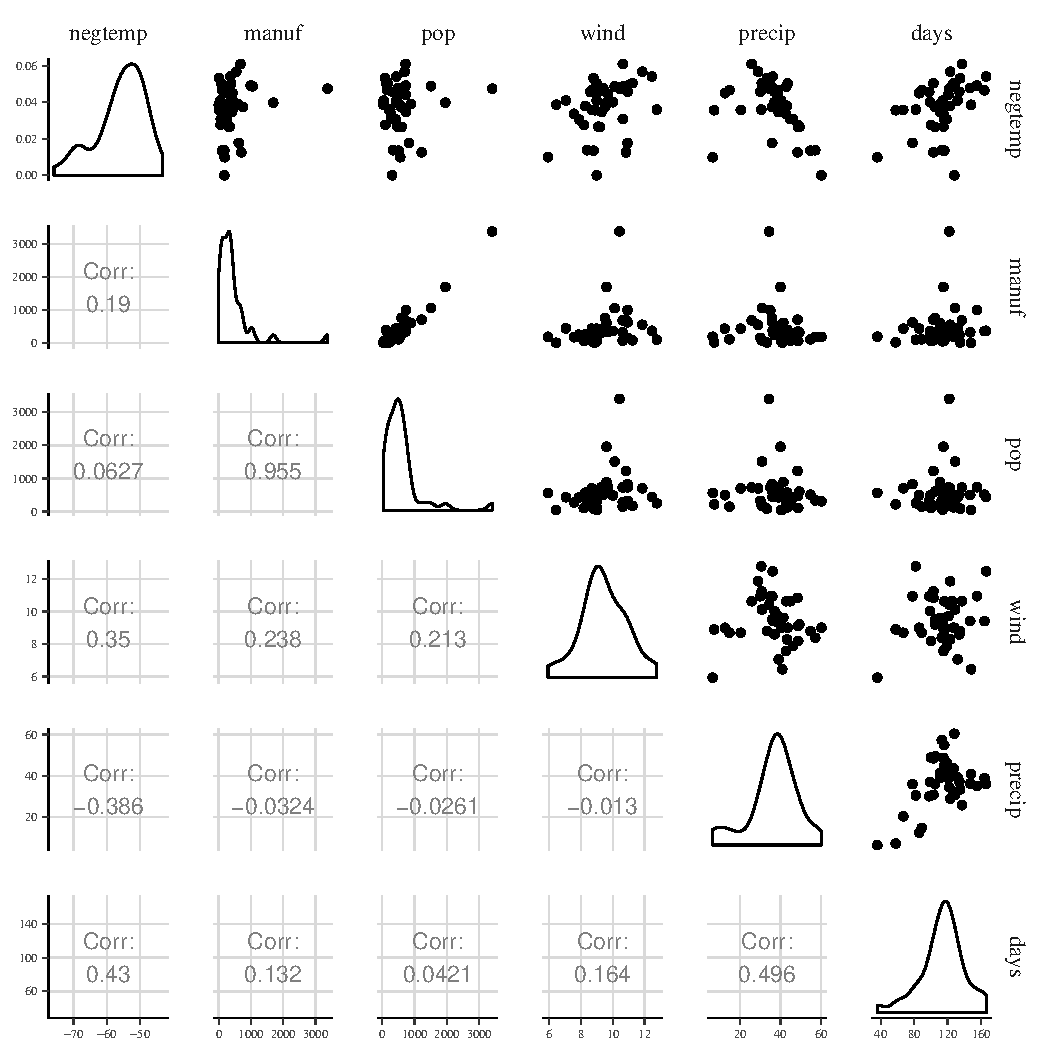
\includegraphics[width=\maxwidth]{figure/ch03_figunnamed-chunk-1-1} 


A simple linear regression model including the dependent variable SO2 and the six explanatory variables is fitted with the lm command in R. The $R^2$ of the full model is 0.670. 

\begin{knitrout}
\definecolor{shadecolor}{rgb}{0.969, 0.969, 0.969}\color{fgcolor}\begin{kframe}
\begin{alltt}
\hlstd{usair.lm} \hlkwb{<-} \hlkwd{lm}\hlstd{(SO2}\hlopt{~}\hlstd{.,} \hlkwc{data} \hlstd{= usair)}


\hlcom{#Code assuming stochastic predictors}
\hlstd{run}\hlkwb{<-}\hlkwd{boot.relimp}\hlstd{(usair.lm,} \hlkwc{fixed}\hlstd{=}\hlnum{TRUE}\hlstd{)}

\hlkwd{booteval.relimp}\hlstd{(run,} \hlkwc{bty} \hlstd{=} \hlstr{"perc"}\hlstd{,} \hlkwc{level} \hlstd{=} \hlnum{0.95}\hlstd{,}
                \hlkwc{sort} \hlstd{=} \hlnum{FALSE}\hlstd{,} \hlkwc{norank} \hlstd{=} \hlnum{TRUE}\hlstd{,} \hlkwc{nodiff} \hlstd{=} \hlnum{TRUE}\hlstd{,}
                \hlkwc{typesel} \hlstd{=} \hlkwd{c}\hlstd{(}\hlstr{"lmg"}\hlstd{))}
\end{alltt}
\begin{verbatim}
## Response variable: SO2 
## Total response variance: 550.9476 
## Analysis based on 41 observations 
## 
## 6 Regressors: 
## negtemp manuf pop wind precip days 
## Proportion of variance explained by model: 66.95%
## Metrics are not normalized (rela=FALSE). 
## 
## Relative importance metrics: 
## 
##                lmg
## negtemp 0.11112440
## manuf   0.29645486
## pop     0.16612543
## wind    0.01670048
## precip  0.01867491
## days    0.06043172
## 
## Average coefficients for different model sizes: 
## 
##                 1X          2Xs          3Xs         4Xs         5Xs
## negtemp 1.40813251  1.334422627  1.281176139  1.25765114  1.28261316
## manuf   0.02685872  0.037288506  0.046426172  0.05392217  0.05982752
## pop     0.02001359  0.004397813 -0.009249699 -0.02072002 -0.03035031
## wind    1.55574078 -0.024806053 -1.384826041 -2.37946774 -2.98034367
## precip  0.10826200  0.114668437  0.164271600  0.26014506  0.40567633
## days    0.32726028  0.297872739  0.241114488  0.15574609  0.04248847
##                 6Xs
## negtemp  1.26794109
## manuf    0.06491817
## pop     -0.03927674
## wind    -3.18136579
## precip   0.51235896
## days    -0.05205019
## 
##  
##  Confidence interval information ( 1000 bootstrap replicates, bty= perc ): 
## Relative Contributions with confidence intervals: 
##  
##                        Lower  Upper
##             percentage 0.95   0.95  
## negtemp.lmg 0.1111     0.0395 0.2157
## manuf.lmg   0.2965     0.2031 0.4133
## pop.lmg     0.1661     0.1137 0.2405
## wind.lmg    0.0167     0.0088 0.0686
## precip.lmg  0.0187     0.0074 0.0658
## days.lmg    0.0604     0.0221 0.1436
## 
## CAUTION: Bootstrap confidence intervals can be somewhat liberal. 
## NOTE: X-matrix has been considered as fixed for bootstrapping.
\end{verbatim}
\begin{alltt}
\hlstd{bayes.usair} \hlkwb{<-} \hlkwd{stan_glm}\hlstd{(SO2} \hlopt{~} \hlstd{. ,}
                  \hlkwc{data} \hlstd{= usair,}
                  \hlkwc{chains} \hlstd{=} \hlnum{4}\hlstd{,} \hlkwc{cores} \hlstd{=} \hlnum{4}\hlstd{)}

\hlcom{#posterior sample}
\hlstd{post.sample} \hlkwb{<-} \hlkwd{as.matrix}\hlstd{(bayes.usair)}

\hlcom{#example of the first 10 posterior samples}
\hlstd{post.sample[}\hlnum{1}\hlopt{:}\hlnum{10}\hlstd{,]}
\end{alltt}
\begin{verbatim}
##           parameters
## iterations (Intercept)   negtemp      manuf          pop        wind
##       [1,]    76.63403 0.9372802 0.04841073 -0.023218029 -2.64495618
##       [2,]   125.55302 1.2466290 0.09637679 -0.066305907 -3.19036264
##       [3,]    57.36694 0.9911093 0.03160349 -0.009311882  0.01044934
##       [4,]    84.42258 1.4791986 0.03711957 -0.014665873 -0.34841785
##       [5,]    93.21212 1.2233823 0.03128086 -0.008084000  0.33863006
##       [6,]    87.03184 1.5349165 0.00412235  0.012872617 -2.55050086
##       [7,]    94.75793 0.7006997 0.05364753 -0.031105908 -3.31781375
##       [8,]    83.86657 0.7426624 0.04801954 -0.025619233 -1.38722141
##       [9,]   102.88610 1.4435390 0.05184942 -0.025740406 -1.64110264
##      [10,]   118.68871 1.0830053 0.05654027 -0.029810740 -5.16775861
##           parameters
## iterations     precip         days    sigma
##       [1,]  0.1604472  0.118589312 13.37797
##       [2,]  0.5069793 -0.137335376 14.59451
##       [3,]  0.5041612 -0.005711373 14.32118
##       [4,]  0.4686286  0.039197926 14.92060
##       [5,]  0.2656314 -0.159223921 15.44457
##       [6,]  0.5662126  0.185683615 16.19240
##       [7,] -0.1457218  0.051595750 14.96856
##       [8,]  0.3112843 -0.139255549 14.45331
##       [9,]  0.2724058  0.048202080 14.16934
##      [10,]  0.2932432  0.029287718 12.75397
\end{verbatim}
\begin{alltt}
\hlcom{#no need for the intercept, last parameter is sigma}
\hlstd{post.sample} \hlkwb{<-} \hlstd{post.sample[,}\hlopt{-}\hlnum{1}\hlstd{]}

\hlcom{#data frame with all submodels}
\hlstd{df.rtwos} \hlkwb{<-}\hlkwd{rtwos}\hlstd{(usair[,}\hlnum{2}\hlopt{:}\hlnum{7}\hlstd{], post.sample)}

\hlstd{df.rtwos[,}\hlnum{1}\hlopt{:}\hlnum{3}\hlstd{]}
\end{alltt}
\begin{verbatim}
##                          X1           X2         X3
## none           0.0000000000 0.000000e+00 0.00000000
## x1             0.2095431804 1.775796e-01 0.13489062
## x2             0.4446934425 4.179614e-01 0.41661681
## x3             0.2929164865 2.203668e-01 0.30988091
## x4             0.0142179243 9.678623e-03 0.06630532
## x5             0.0002332062 3.691272e-07 0.01541407
## x6             0.1708118912 8.639088e-02 0.13975755
## x1 x2          0.5583792612 5.104269e-01 0.47869292
## x1 x3          0.4732622423 3.746202e-01 0.42079549
## x1 x4          0.2114451600 1.803153e-01 0.15386482
## x1 x5          0.2529084140 2.084866e-01 0.21806295
## x1 x6          0.2669814140 1.931435e-01 0.19205192
## x2 x3          0.5496435031 6.689090e-01 0.45766492
## x2 x4          0.4463420384 4.212209e-01 0.42806286
## x2 x5          0.4460556275 4.183760e-01 0.43768634
## x2 x6          0.5524401553 4.622856e-01 0.50146874
## x3 x4          0.2929345455 2.203690e-01 0.33015361
## x3 x5          0.2937818488 2.205027e-01 0.32912977
## x3 x6          0.4456911919 2.956683e-01 0.43288956
## x4 x5          0.0145009021 9.679073e-03 0.08256418
## x4 x6          0.1735285646 8.897505e-02 0.17929668
## x5 x6          0.2185774367 1.148293e-01 0.14474330
## x1 x2 x3       0.5999081239 6.806839e-01 0.49085217
## x1 x2 x4       0.5828622187 5.369044e-01 0.47953024
## x1 x2 x5       0.5913931426 5.328805e-01 0.54740304
## x1 x2 x6       0.6010744974 5.189484e-01 0.52124884
## x1 x3 x4       0.4962294308 3.959121e-01 0.42165365
## x1 x3 x5       0.5170723418 4.058519e-01 0.50460899
## x1 x3 x6       0.5266597023 3.883851e-01 0.47376230
## x1 x4 x5       0.2583510585 2.145589e-01 0.22766353
## x1 x4 x6       0.2692358837 1.960944e-01 0.20998386
## x1 x5 x6       0.2678265140 2.091053e-01 0.21831904
## x2 x3 x4       0.5529165888 6.757592e-01 0.46702982
## x2 x3 x5       0.5514266268 6.697259e-01 0.47971614
## x2 x3 x6       0.6100903238 6.738347e-01 0.51696588
## x2 x4 x5       0.4476880079 4.216230e-01 0.44930231
## x2 x4 x6       0.5599544061 4.698455e-01 0.50602109
## x2 x5 x6       0.5747343757 4.722065e-01 0.50147391
## x3 x4 x5       0.2938018636 2.205046e-01 0.34970572
## x3 x4 x6       0.4491269234 2.977539e-01 0.44059086
## x3 x5 x6       0.4819547629 3.164232e-01 0.43459853
## x4 x5 x6       0.2193728852 1.158819e-01 0.18169678
## x1 x2 x3 x4    0.6190277770 6.963630e-01 0.49239417
## x1 x2 x3 x5    0.6222290346 6.872889e-01 0.55188213
## x1 x2 x3 x6    0.6323045906 6.819204e-01 0.52802696
## x1 x2 x4 x5    0.6247895508 5.669954e-01 0.54744668
## x1 x2 x4 x6    0.6259280279 5.455982e-01 0.52201955
## x1 x2 x5 x6    0.6019013867 5.348317e-01 0.54741474
## x1 x3 x4 x5    0.5508487894 4.358934e-01 0.50477150
## x1 x3 x4 x6    0.5505484630 4.101271e-01 0.47445457
## x1 x3 x5 x6    0.5284278757 4.073263e-01 0.50460907
## x1 x4 x5 x6    0.2708395551 2.159926e-01 0.22869636
## x2 x3 x4 x5    0.5546775480 6.765545e-01 0.48921418
## x2 x3 x4 x6    0.6181232920 6.824053e-01 0.52131583
## x2 x3 x5 x6    0.6210337734 6.739417e-01 0.51746614
## x2 x4 x5 x6    0.5847711002 4.814350e-01 0.50603453
## x3 x4 x5 x6    0.4880867456 3.200922e-01 0.44165482
## x1 x2 x3 x4 x5 0.6488611356 7.067140e-01 0.55188379
## x1 x2 x3 x4 x6 0.6523787469 6.977712e-01 0.52929783
## x1 x2 x3 x5 x6 0.6324408123 6.895395e-01 0.55189795
## x1 x2 x4 x5 x6 0.6300577358 5.728615e-01 0.54746790
## x1 x3 x4 x5 x6 0.5566788981 4.406473e-01 0.50477765
## x2 x3 x4 x5 x6 0.6308577065 6.827467e-01 0.52211213
## all            0.6544018382 7.119186e-01 0.55189833
\end{verbatim}
\begin{alltt}
\hlcom{# prepare data frame for LMG values}

\hlstd{LMG.Vals}\hlkwb{<-}\hlkwd{matrix}\hlstd{(}\hlnum{0}\hlstd{,} \hlnum{6}\hlstd{,} \hlkwd{dim}\hlstd{(df.rtwos)[}\hlnum{2}\hlstd{])}

\hlkwa{for}\hlstd{(i} \hlkwa{in} \hlnum{1}\hlopt{:}\hlkwd{dim}\hlstd{(df.rtwos)[}\hlnum{2}\hlstd{])\{}

  \hlstd{gofn}\hlkwb{<-}\hlstd{df.rtwos[,i]}

  \hlstd{obj.Gelman}\hlkwb{<-}\hlkwd{partition}\hlstd{(gofn,} \hlkwc{pcan} \hlstd{=} \hlnum{6}\hlstd{,} \hlkwc{var.names} \hlstd{=} \hlkwd{names}\hlstd{(usair[,}\hlnum{2}\hlopt{:}\hlnum{7}\hlstd{]))}

  \hlstd{LMG.Vals[,i]}\hlkwb{=}\hlstd{obj.Gelman}\hlopt{$}\hlstd{IJ[,}\hlnum{1}\hlstd{]}
\hlstd{\}}

\hlcom{# posterior LMG distribution of each variable}
\hlkwd{quantile}\hlstd{(LMG.Vals[}\hlnum{1}\hlstd{,],} \hlkwd{c}\hlstd{(}\hlnum{0.025}\hlstd{,} \hlnum{0.5}\hlstd{,} \hlnum{0.975}\hlstd{))}
\end{alltt}
\begin{verbatim}
##       2.5%        50%      97.5% 
## 0.03140146 0.10425536 0.20332655
\end{verbatim}
\begin{alltt}
\hlkwd{quantile}\hlstd{(LMG.Vals[}\hlnum{2}\hlstd{,],} \hlkwd{c}\hlstd{(}\hlnum{0.025}\hlstd{,} \hlnum{0.5}\hlstd{,} \hlnum{0.975}\hlstd{))}
\end{alltt}
\begin{verbatim}
##      2.5%       50%     97.5% 
## 0.1528304 0.2641768 0.3565642
\end{verbatim}
\begin{alltt}
\hlkwd{quantile}\hlstd{(LMG.Vals[}\hlnum{3}\hlstd{,],} \hlkwd{c}\hlstd{(}\hlnum{0.025}\hlstd{,} \hlnum{0.5}\hlstd{,} \hlnum{0.975}\hlstd{))}
\end{alltt}
\begin{verbatim}
##       2.5%        50%      97.5% 
## 0.08782959 0.15190153 0.21056465
\end{verbatim}
\begin{alltt}
\hlkwd{quantile}\hlstd{(LMG.Vals[}\hlnum{4}\hlstd{,],} \hlkwd{c}\hlstd{(}\hlnum{0.025}\hlstd{,} \hlnum{0.5}\hlstd{,} \hlnum{0.975}\hlstd{))}
\end{alltt}
\begin{verbatim}
##        2.5%         50%       97.5% 
## 0.007501645 0.017654467 0.071564974
\end{verbatim}
\begin{alltt}
\hlkwd{quantile}\hlstd{(LMG.Vals[}\hlnum{5}\hlstd{,],} \hlkwd{c}\hlstd{(}\hlnum{0.025}\hlstd{,} \hlnum{0.5}\hlstd{,} \hlnum{0.975}\hlstd{))}
\end{alltt}
\begin{verbatim}
##        2.5%         50%       97.5% 
## 0.006988704 0.020612799 0.069884355
\end{verbatim}
\begin{alltt}
\hlkwd{quantile}\hlstd{(LMG.Vals[}\hlnum{6}\hlstd{,],} \hlkwd{c}\hlstd{(}\hlnum{0.025}\hlstd{,} \hlnum{0.5}\hlstd{,} \hlnum{0.975}\hlstd{))}
\end{alltt}
\begin{verbatim}
##       2.5%        50%      97.5% 
## 0.01761491 0.05739723 0.13408836
\end{verbatim}
\begin{alltt}
\hlcom{#Visualization}
\hlstd{dat} \hlkwb{<-} \hlkwd{data.frame}\hlstd{(}\hlkwd{t}\hlstd{(LMG.Vals))}

\hlstd{pairs.chart} \hlkwb{<-} \hlkwd{ggpairs}\hlstd{(dat,} \hlkwc{lower} \hlstd{=} \hlkwd{list}\hlstd{(}\hlkwd{list}\hlstd{(}\hlkwc{combo} \hlstd{=} \hlstr{"facetdensity"}\hlstd{)),} \hlkwc{upper} \hlstd{=} \hlkwd{list}\hlstd{(}\hlkwd{list}\hlstd{(}\hlkwc{continuous} \hlstd{=} \hlstr{"cor"}\hlstd{)))} \hlopt{+} \hlstd{ggplot2}\hlopt{::}\hlkwd{theme}\hlstd{(}\hlkwc{axis.text} \hlstd{=} \hlkwd{element_text}\hlstd{(}\hlkwc{size} \hlstd{=} \hlnum{6}\hlstd{))}
\hlstd{pairs.chart}
\end{alltt}
\end{kframe}
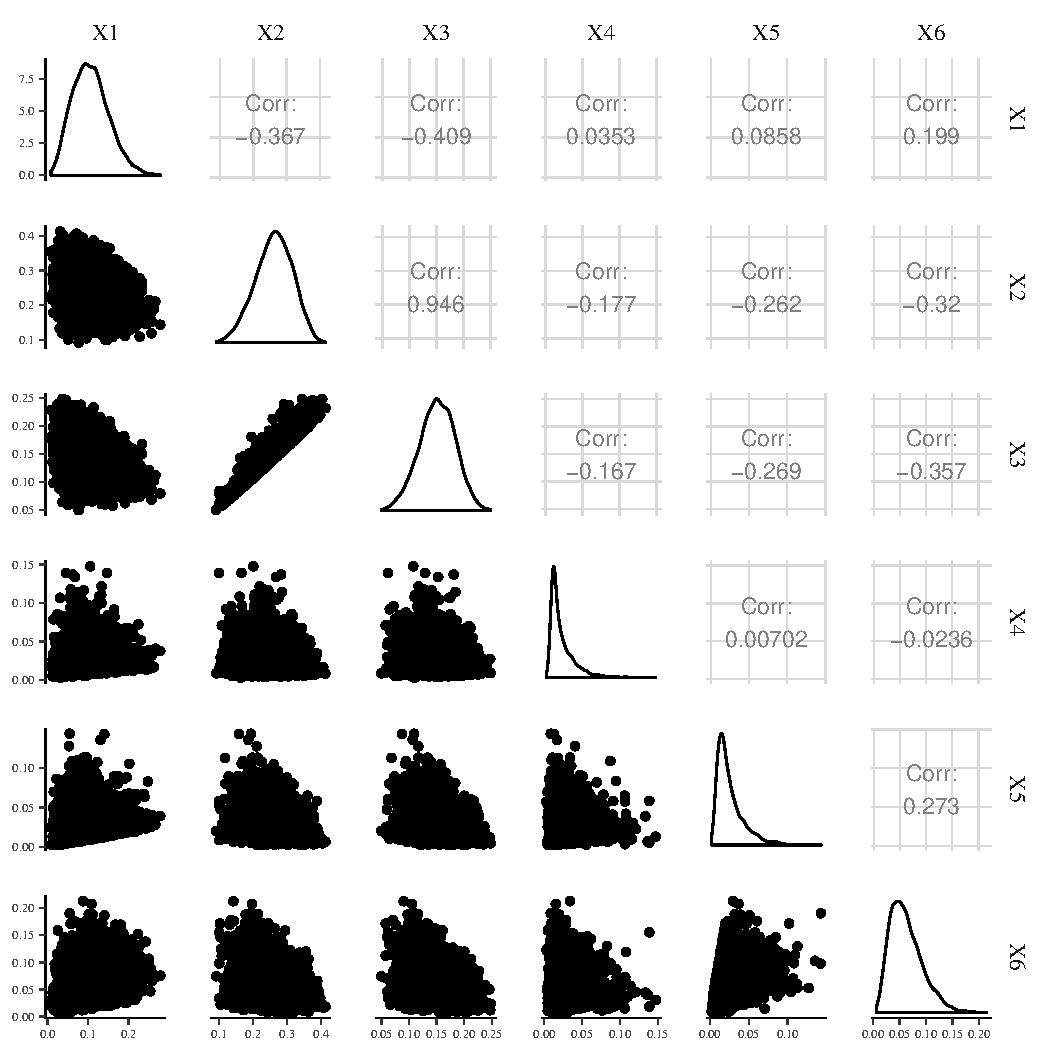
\includegraphics[width=\maxwidth]{figure/ch03_figreal_data_LMG-1} 
\begin{kframe}\begin{alltt}
\hlcom{#use prior knowledge}
\hlstd{my_prior} \hlkwb{<-} \hlkwd{normal}\hlstd{(}\hlkwc{location} \hlstd{=} \hlkwd{c}\hlstd{(}\hlnum{1}\hlstd{,} \hlnum{0.05}\hlstd{,}\hlopt{-}\hlnum{0.03}\hlstd{,}\hlopt{-}\hlnum{3}\hlstd{,} \hlnum{0}\hlstd{,} \hlnum{0}\hlstd{),} \hlkwc{scale} \hlstd{=} \hlkwd{c}\hlstd{(}\hlnum{0.1}\hlstd{,} \hlnum{0.01}\hlstd{,}\hlnum{0.01}\hlstd{,}\hlnum{0.1}\hlstd{,} \hlnum{0.1}\hlstd{,} \hlnum{0.1}\hlstd{),} \hlkwc{autoscale} \hlstd{=} \hlnum{FALSE}\hlstd{)}


\hlstd{bayes.usair} \hlkwb{<-} \hlkwd{stan_glm}\hlstd{(SO2} \hlopt{~} \hlstd{. ,}
                  \hlkwc{data} \hlstd{= usair,} \hlkwc{prior} \hlstd{= my_prior,}
                  \hlkwc{chains} \hlstd{=} \hlnum{4}\hlstd{,} \hlkwc{cores} \hlstd{=} \hlnum{4}\hlstd{)}

\hlcom{#posterior sample}
\hlstd{post.sample} \hlkwb{<-} \hlkwd{as.matrix}\hlstd{(bayes.usair)}

\hlcom{#example of the first 10 posterior samples}
\hlstd{post.sample[}\hlnum{1}\hlopt{:}\hlnum{10}\hlstd{,]}
\end{alltt}
\begin{verbatim}
##           parameters
## iterations (Intercept)   negtemp      manuf         pop      wind
##       [1,]    89.81921 0.9954251 0.04757398 -0.01827321 -2.874278
##       [2,]   102.34929 0.8576861 0.05986172 -0.04000167 -3.068902
##       [3,]    82.48015 0.8726391 0.06028279 -0.02943372 -2.886816
##       [4,]   104.68428 1.1246337 0.06291728 -0.02986882 -2.992389
##       [5,]   105.32564 1.0099265 0.06004396 -0.03390757 -3.042098
##       [6,]    97.62453 0.9849631 0.05775336 -0.03569145 -3.181789
##       [7,]   108.99691 1.1103095 0.06485238 -0.03683087 -3.038839
##       [8,]   108.00249 1.1095669 0.06392837 -0.03489973 -3.022639
##       [9,]   104.88886 0.8596561 0.06802693 -0.04236175 -3.114606
##      [10,]   110.01475 1.0939596 0.03827552 -0.01521879 -2.874750
##           parameters
## iterations       precip         days    sigma
##       [1,]  0.276227708  0.012587472 15.36679
##       [2,] -0.083183938  0.032998990 17.82745
##       [3,]  0.059481326  0.090567911 11.39204
##       [4,]  0.166154108 -0.005130413 15.37028
##       [5,] -0.005799239  0.011521322 15.34251
##       [6,]  0.078044836  0.044796613 18.45930
##       [7,]  0.224391786 -0.076565709 16.99801
##       [8,]  0.233775974 -0.075735576 17.02467
##       [9,]  0.017462691 -0.001904609 14.16142
##      [10,] -0.019851667 -0.010796473 15.93392
\end{verbatim}
\begin{alltt}
\hlcom{#no need for the intercept, last parameter is sigma}
\hlstd{post.sample} \hlkwb{<-} \hlstd{post.sample[,}\hlopt{-}\hlnum{1}\hlstd{]}

\hlcom{#data frame with all submodels}
\hlstd{df.rtwos} \hlkwb{<-}\hlkwd{rtwos}\hlstd{(usair[,}\hlnum{2}\hlopt{:}\hlnum{7}\hlstd{], post.sample)}


\hlcom{# prepare data frame for LMG values}

\hlstd{LMG.Vals}\hlkwb{<-}\hlkwd{matrix}\hlstd{(}\hlnum{0}\hlstd{,} \hlnum{6}\hlstd{,} \hlkwd{dim}\hlstd{(df.rtwos)[}\hlnum{2}\hlstd{])}

\hlkwa{for}\hlstd{(i} \hlkwa{in} \hlnum{1}\hlopt{:}\hlkwd{dim}\hlstd{(df.rtwos)[}\hlnum{2}\hlstd{])\{}

  \hlstd{gofn}\hlkwb{<-}\hlstd{df.rtwos[,i]}

  \hlstd{obj.Gelman}\hlkwb{<-}\hlkwd{partition}\hlstd{(gofn,} \hlkwc{pcan} \hlstd{=} \hlnum{6}\hlstd{,} \hlkwc{var.names} \hlstd{=} \hlkwd{names}\hlstd{(usair[,}\hlnum{2}\hlopt{:}\hlnum{7}\hlstd{]))}

  \hlstd{LMG.Vals[,i]}\hlkwb{=}\hlstd{obj.Gelman}\hlopt{$}\hlstd{IJ[,}\hlnum{1}\hlstd{]}
\hlstd{\}}

\hlcom{# posterior LMG distribution of each variable}
\hlkwd{quantile}\hlstd{(LMG.Vals[}\hlnum{1}\hlstd{,],} \hlkwd{c}\hlstd{(}\hlnum{0.025}\hlstd{,} \hlnum{0.5}\hlstd{,} \hlnum{0.975}\hlstd{))}
\end{alltt}
\begin{verbatim}
##       2.5%        50%      97.5% 
## 0.07362282 0.11363424 0.16192618
\end{verbatim}
\begin{alltt}
\hlkwd{quantile}\hlstd{(LMG.Vals[}\hlnum{2}\hlstd{,],} \hlkwd{c}\hlstd{(}\hlnum{0.025}\hlstd{,} \hlnum{0.5}\hlstd{,} \hlnum{0.975}\hlstd{))}
\end{alltt}
\begin{verbatim}
##      2.5%       50%     97.5% 
## 0.1695037 0.2591710 0.3325388
\end{verbatim}
\begin{alltt}
\hlkwd{quantile}\hlstd{(LMG.Vals[}\hlnum{3}\hlstd{,],} \hlkwd{c}\hlstd{(}\hlnum{0.025}\hlstd{,} \hlnum{0.5}\hlstd{,} \hlnum{0.975}\hlstd{))}
\end{alltt}
\begin{verbatim}
##       2.5%        50%      97.5% 
## 0.09346488 0.15095056 0.20686893
\end{verbatim}
\begin{alltt}
\hlkwd{quantile}\hlstd{(LMG.Vals[}\hlnum{4}\hlstd{,],} \hlkwd{c}\hlstd{(}\hlnum{0.025}\hlstd{,} \hlnum{0.5}\hlstd{,} \hlnum{0.975}\hlstd{))}
\end{alltt}
\begin{verbatim}
##       2.5%        50%      97.5% 
## 0.01262413 0.01637030 0.02123865
\end{verbatim}
\begin{alltt}
\hlkwd{quantile}\hlstd{(LMG.Vals[}\hlnum{5}\hlstd{,],} \hlkwd{c}\hlstd{(}\hlnum{0.025}\hlstd{,} \hlnum{0.5}\hlstd{,} \hlnum{0.975}\hlstd{))}
\end{alltt}
\begin{verbatim}
##        2.5%         50%       97.5% 
## 0.007893674 0.013095342 0.025689887
\end{verbatim}
\begin{alltt}
\hlkwd{quantile}\hlstd{(LMG.Vals[}\hlnum{6}\hlstd{,],} \hlkwd{c}\hlstd{(}\hlnum{0.025}\hlstd{,} \hlnum{0.5}\hlstd{,} \hlnum{0.975}\hlstd{))}
\end{alltt}
\begin{verbatim}
##       2.5%        50%      97.5% 
## 0.01733809 0.05146921 0.10703968
\end{verbatim}
\begin{alltt}
\hlcom{#Visualization}
\hlstd{dat} \hlkwb{<-} \hlkwd{data.frame}\hlstd{(}\hlkwd{t}\hlstd{(LMG.Vals))}

\hlstd{pairs.chart} \hlkwb{<-} \hlkwd{ggpairs}\hlstd{(dat,} \hlkwc{lower} \hlstd{=} \hlkwd{list}\hlstd{(}\hlkwd{list}\hlstd{(}\hlkwc{combo} \hlstd{=} \hlstr{"facetdensity"}\hlstd{)),} \hlkwc{upper} \hlstd{=} \hlkwd{list}\hlstd{(}\hlkwd{list}\hlstd{(}\hlkwc{continuous} \hlstd{=} \hlstr{"cor"}\hlstd{)))} \hlopt{+} \hlstd{ggplot2}\hlopt{::}\hlkwd{theme}\hlstd{(}\hlkwc{axis.text} \hlstd{=} \hlkwd{element_text}\hlstd{(}\hlkwc{size} \hlstd{=} \hlnum{6}\hlstd{))}
\hlstd{pairs.chart}
\end{alltt}
\end{kframe}
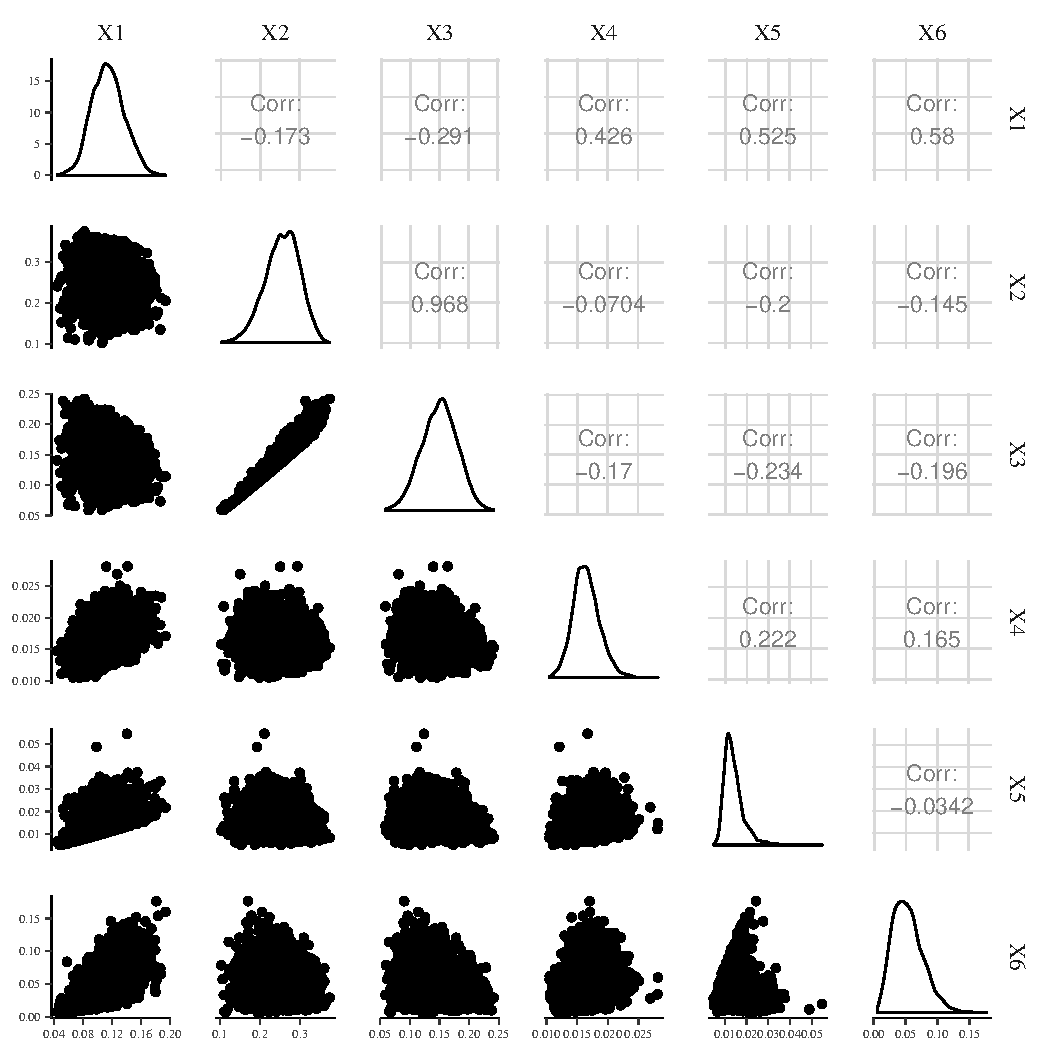
\includegraphics[width=\maxwidth]{figure/ch03_figreal_data_LMG-2} 

\end{knitrout}




\bibliographystyle{mywiley} 
\bibliography{biblio}
\end{document}
